%=====================================================================
%  NinaivX — MSc Dissertation (Chapters 1–8: complete, incl. Evaluation)
%  Ashwin Kumar Ramesh Kumar · MSc Artificial Intelligence
%  University of Sheffield
%
%  Compile:  pdflatex NinaivX-Report.tex   (run twice for the ToC/refs)
%  Images:   drop your figures into ./figures/ and replace the
%            placeholders marked  % TODO IMAGE
%=====================================================================
\documentclass[11pt,a4paper]{report}

\usepackage[utf8]{inputenc}
\usepackage[T1]{fontenc}
\usepackage{lmodern}
% Binding-friendly margins per the departmental guidelines (left 37mm for the
% binding edge, right 25mm), with room for the running header.
\usepackage[top=25mm,bottom=25mm,left=37mm,right=25mm,headheight=15pt,headsep=10pt]{geometry}
\usepackage{amsmath}
\usepackage{amssymb}   % \checkmark, \circleddash, \lozenge used in the status tables
\usepackage{graphicx}
\usepackage{booktabs}
\usepackage{tabularx}
\usepackage{array}
\usepackage{xcolor}
\usepackage{caption}
\usepackage{setspace}
\usepackage{enumitem}
\usepackage{float}
\usepackage[hidelinks]{hyperref}
\usepackage{fancyhdr}

\graphicspath{{figures/}}
\captionsetup{font=small,labelfont=bf}
% Line spacing per the guidelines (single/1.1/1.2): 1.15.
\setstretch{1.15}
\setlength{\parskip}{0.4em}

% Running header: chapter (or appendix) title centred at the top of every page,
% page number centred at the foot, so all pages are numbered.
\pagestyle{fancy}
\fancyhf{}
\makeatletter
\renewcommand{\chaptermark}[1]{\markboth{\@chapapp\ \thechapter.\ #1}{}}
\makeatother
\fancyhead[C]{\small\nouppercase{\leftmark}}
\fancyfoot[C]{\thepage}
\renewcommand{\headrulewidth}{0.4pt}
\renewcommand{\footrulewidth}{0pt}
% Chapter-opening pages (plain style) still get a centred page number.
\fancypagestyle{plain}{%
  \fancyhf{}%
  \fancyfoot[C]{\thepage}%
  \renewcommand{\headrulewidth}{0pt}%
}

% Convenience command for the (very common) missing-figure placeholders.
% Usage: \placeholder{description}{caption}{fig:label}
% Replace with a real \includegraphics (keeping the same \label) when the image is ready.
\newcommand{\placeholder}[3]{%
  \begin{figure}[H]\centering
    \fbox{\parbox[c][4.5cm][c]{0.8\linewidth}{\centering\itshape
      [ Figure placeholder: #1 ]\\[2pt]\small (add your image to ./figures/ and use \texttt{\textbackslash includegraphics})}}
    \caption{#2}\label{#3}
  \end{figure}}

% Renders the image if it exists (checking BOTH figures/ and the project root,
% so it works wherever you upload it), else a labelled placeholder box, so the
% document always compiles and auto-upgrades the moment you drop the file in.
% Usage: \imgorph{file.png}  or  \imgorph[0.45\linewidth]{file.png}
\newcommand{\imgorph}[2][\linewidth]{%
  \IfFileExists{figures/#2}%
    {\includegraphics[width=#1]{figures/#2}}%
    {\IfFileExists{#2}%
      {\includegraphics[width=#1]{#2}}%
      {\fbox{\parbox[c][3.6cm][c]{\dimexpr#1-2\fboxsep-2\fboxrule\relax}{\centering\itshape [\,add \texttt{#2}\\ (in the \texttt{figures/} folder)\,]}}}}}

\begin{document}

%=====================================================================
% TITLE PAGE
%=====================================================================
\begin{titlepage}
\centering
\vspace*{1cm}
{\large University of Sheffield\par}
\vspace{1.5cm}
{\LARGE\bfseries NinaivX: Designing and Evaluating a Privacy-First,\\[4pt]
Dual-Mode Voice Conversational AI for\\[4pt]
Bereavement Support and Companionship\par}
\vspace{2cm}

% Optional: add figures/sheffield-logo.png for the University crest.
\imgorph[0.28\linewidth]{sheffield-logo.png}
\vspace{1.5cm}

{\large Ashwin Kumar Ramesh Kumar\par}
\vspace{0.5cm}
{\normalsize Supervisor: \emph{[Supervisor name]}\par}
\vspace{1.5cm}
{\normalsize A dissertation submitted in partial fulfilment of the requirements\\
for the degree of MSc in Artificial Intelligence\\[4pt]
in the\\[4pt]
Department of Computer Science\par}
\vfill
{\normalsize \today\par}
\end{titlepage}

% Front matter numbered in roman; plain style (page number only, no chapter header).
\pagenumbering{roman}
\pagestyle{plain}

%=====================================================================
% ABSTRACT
%=====================================================================
\chapter*{Abstract}
\addcontentsline{toc}{chapter}{Abstract}

Grief and loneliness are widespread and serious public-health concerns: the World Health Organization estimates that around one in six people worldwide are affected by loneliness, a condition linked to an estimated 871{,}000 deaths every year. In parallel, a commercial ``digital afterlife industry'' has begun to offer conversational recreations of the dead, demonstrating genuine demand but also raising acute ethical risks around factual fabrication, consent, transparency and dependency. This dissertation presents \emph{NinaivX}, a privacy-first, dual-mode voice conversational AI designed to explore how such a system can be made emotionally supportive, factually safer and privacy-respecting.

NinaivX offers two personas behind a single architecture. A \emph{Companion} mode provides a living, web-connected AI friend intended to ease loneliness, while a \emph{Legacy} mode allows a bereaved user to hold a gentle spoken conversation with an AI recreation of a loved one who has passed away. The central design idea is safety by construction: the Legacy persona is deliberately \emph{air-gapped} from the internet and grounded only in the information the user provides, so that it cannot pull in and repeat fabricated ``news'' about the real person. A supervisor router directs each conversation to the correct persona, giving each mode its own capability and safety profile. The system is implemented as a FastAPI backend orchestrated with LangGraph over AWS Bedrock (Claude), an ElevenLabs voice pipeline for speech-to-text, text-to-speech and voice cloning, Supabase for authentication and storage, and a React Native (Expo) mobile client.

The design was validated through structured safety testing --- confirming that the air-gap, per-user isolation, content policy and temporal grounding hold in the running system --- and evaluated empirically through a remote, anonymous user study of twenty-one adult participants that received formal University ethical approval. Participants rated the experience highly across usability, conversational quality, safety and comfort (an overall mean of 4.6 on a five-point scale, with every respondent agreeing that the system was easy to use, that they felt comfortable, and that they were satisfied overall), while identifying the naturalness of the synthesised voice as the clearest target for improvement. A separate controlled experiment, comparing the design against an unconstrained baseline on the same model, found that the grounding cut the fabrication rate on fabrication-prone questions from 83\% to 28\% and all but eliminated fabrication about events after the person's death, at no measured cost to conversational quality. Together the results support the central claim that a dual-mode, safety-by-construction design can be made emotionally supportive and factually safer without sacrificing perceived conversational quality.

%=====================================================================
% DECLARATION
%=====================================================================
\chapter*{Declaration}
\addcontentsline{toc}{chapter}{Declaration}
I declare that this dissertation is my own work, carried out as part of the MSc in Artificial Intelligence at the University of Sheffield. All external sources of information have been acknowledged and referenced. This work has not been submitted for any other degree.
\vspace{2cm}

\noindent Signed: \underline{\hspace{6cm}} \qquad Date: \underline{\hspace{3cm}}

%=====================================================================
% ACKNOWLEDGEMENTS
%=====================================================================
\chapter*{Acknowledgements}
\addcontentsline{toc}{chapter}{Acknowledgements}
% TODO: personalise — supervisor, family, participants, etc.
I would like to thank my supervisor for their guidance throughout this project, and everyone who gave their time to test the application and share feedback.

\tableofcontents
\listoffigures
\listoftables

% Body numbered in arabic from Chapter 1; running chapter header restored.
\cleardoublepage
\pagenumbering{arabic}
\pagestyle{fancy}

%=====================================================================
% CHAPTER 1 — INTRODUCTION
%=====================================================================
\chapter{Introduction}
\label{ch:intro}

\section{Problem and motivation}
The loss of a loved one and the experience of chronic loneliness are among the most universal forms of human suffering, and both are unusually widespread today. In its 2025 report the World Health Organization's Commission on Social Connection estimated that around one in six people worldwide are affected by loneliness, and that social isolation and loneliness are associated with roughly 871{,}000 deaths per year \cite{who2025loneliness}. When someone close to us dies, we are typically left with photographs, recordings and written messages, but with no way to \emph{interact} with the person again --- to hear their voice answer a new question, or to be comforted in their particular way of speaking.

Against this backdrop, a small but growing ``digital afterlife industry'' has begun to commercialise the idea of conversational recreations of the dead \cite{ohman2017political}. Services now exist that will replay a person's consented recordings \cite{hereafter}, or use large language models to generate open-ended conversation in the voice and manner of someone who has passed away \cite{fagone2021jessica,yov}. The very existence of these services confirms a real and deeply human demand. It also, however, exposes a set of serious risks. Modern generative models are fluent but not reliable: they routinely produce confident text that is factually wrong \cite{brown2020language,ji2023survey}. A system that imitates a specific, real, deceased person and invents memories they never had is not merely inaccurate --- it risks distorting a grieving person's memory of the very individual they are trying to hold on to. Alongside this sit questions of consent (the dead cannot agree to be simulated), transparency (does the user know they are speaking to an AI?), and dependency (is the design helping the user grieve, or quietly encouraging them never to let go?).

This project investigates how a voice-based conversational system for the bereaved and the lonely can be designed so that it is \emph{emotionally supportive}, \emph{factually safer}, and \emph{privacy-respecting}, and how such a design compares with the commercial systems and ethical literature that surround it.

\section{Aim}
The aim of this project is to design, implement and evaluate a privacy-first, dual-mode voice conversational AI that (a) supports healthy grieving and companionship, and (b) reduces the risk of factual fabrication when representing a real, deceased person, through an explicit, safety-oriented architecture --- and to critically assess this approach against existing commercial systems and the relevant ethical literature.

\section{Objectives}
The aim is pursued through five objectives:
\begin{enumerate}[itemsep=2pt]
  \item Review the literature on conversational AI, speech synthesis and voice cloning, AI companionship, the digital afterlife industry, and AI safety and ethics, in order to identify the gap this project addresses (Chapter~\ref{ch:background}).
  \item Design a dual-mode architecture comprising an \emph{air-gapped}, retrieval-constrained ``legacy'' (deceased) mode and a \emph{web-connected} ``companion'' mode, mediated by a supervisor router (Chapter~\ref{ch:design}).
  \item Implement the backend and mobile client: agent orchestration, speech-to-text and text-to-speech, persona memory, voice cloning, and secure authentication (Chapter~\ref{ch:impl}).
  \item Test the resulting system, verifying both its functional behaviour and the safety guarantees the design is intended to provide (Chapter~\ref{ch:testing}).
  \item Evaluate the safety design empirically through a user study, and critically discuss the ethical implications --- consent, transparency, and grief support versus grief replacement --- relative to existing systems (Chapter~\ref{ch:eval}).
\end{enumerate}

\section{Research questions}
The project is organised around two research questions:
\begin{description}[leftmargin=2.2em,style=nextline]
  \item[RQ1.] Can an air-gapped, retrieval-constrained design reduce factual fabrication in a voice-based legacy persona compared with an unconstrained generative approach, while maintaining perceived conversational quality?
  \item[RQ2.] How can a single dual-mode architecture satisfy the differing safety and capability requirements of a deceased (legacy) persona and a living (companion) persona?
\end{description}

\section{Contributions}
The contributions of this work are:
\begin{itemize}[itemsep=2pt]
  \item A reproducible, openly documented \textbf{dual-mode architecture} for safety-aware conversational voice AI, in which a single system serves two personas with deliberately different safety and capability profiles.
  \item An explicit \textbf{safety- and privacy-oriented design} --- most notably air-gapping the deceased persona from the internet --- that operationalises, in running code, harms that the ethics literature has so far raised only in the abstract.
  \item A \textbf{critical positioning} of the system against existing commercial offerings, in particular \emph{You, Only Virtual}, including an ethical discussion of grief support versus grief replacement.
  \item An \textbf{empirical evaluation} of the safety design --- the very element that commercial products do not publish --- through an ethics-approved user study, showing that the approach is well received across usability, safety and comfort.
\end{itemize}

\section{Report structure}
Chapter~\ref{ch:background} surveys the relevant literature and derives the gap the project addresses. Chapter~\ref{ch:requirements} turns that gap into a prioritised requirements specification. Chapter~\ref{ch:design} presents the dual-mode design and its safety mechanisms; Chapter~\ref{ch:impl} describes the implementation of the backend and mobile client; and Chapter~\ref{ch:testing} reports the testing of the system's functional and safety behaviour. Chapter~\ref{ch:eval} presents the empirical evaluation --- the safety validation and the user study --- and Chapter~\ref{ch:conclusion} concludes with a reflection against the aims and directions for future work.

%=====================================================================
% CHAPTER 2 — BACKGROUND / LITERATURE SURVEY
%=====================================================================
\chapter{Background and Literature Survey}
\label{ch:background}
\label{ch:lit}

This chapter reviews the fields on which NinaivX draws and against which it is positioned. The project sits at the meeting point of four areas: conversational AI, speech technology, AI companionship, and the emerging digital afterlife industry --- the collective term for commercial services that manage or reconstruct a person's presence after death \cite{abramson2020patent}. The review is organised by topic and, within each topic, moves from the earliest to the most recent work; it closes by identifying the gap that motivates this dissertation.

\section{Conversational AI: from rules to neural language models}
Conversational software is not new. Weizenbaum's \emph{ELIZA} (1966) matched keywords in a user's input to canned response templates, imitating a psychotherapist without any understanding or memory of the conversation \cite{weizenbaum1966eliza}. Strikingly, users attributed genuine feelings to it --- the so-called ``ELIZA effect'' --- a first hint of how readily people anthropomorphise conversational systems, and a caution that is directly relevant to a griefbot.

The modern era began with the \emph{Transformer} \cite{vaswani2017attention}, whose self-attention mechanism replaced recurrent designs and made it possible to train very large language models efficiently. Scaling that architecture produced systems such as GPT-3 \cite{brown2020language}, a 175-billion-parameter model capable of fluent, few-shot generation. Crucially for this project, the same work that demonstrated GPT-3's fluency also documented its tendency to produce confident text that is factually wrong or biased --- the phenomenon later formalised as \emph{hallucination}. A complementary line of work, exemplified by BERT \cite{devlin2019bert}, used bidirectional pre-training to improve language \emph{understanding} (for tasks such as sentiment and intent classification); as an encoder, however, it cannot itself generate spoken replies and therefore serves only as a supporting component. The trajectory of the field is thus one from rigid but predictable rule-based systems to fluent but factually unreliable neural ones --- a tension at the heart of any application that impersonates a real person.

\section{Speech technology: synthesis, recognition and voice cloning}
For a system whose central promise is \emph{voice}, the state of speech technology is decisive. On the synthesis side, Tacotron~2 \cite{shen2018tacotron} brought text-to-speech naturalness close to human recordings (a mean opinion score of 4.53), but produced a single neutral speaking style and could not quickly reproduce a specific person's voice or emotion. On the recognition side, Whisper \cite{radford2023whisper} was trained on around 680{,}000 hours of weakly labelled audio and is robust across accents and noisy conditions, although it is batch-oriented, can hallucinate text during silences, and introduces latency.

Two developments make personalised voice practical --- and ethically fraught. VALL-E \cite{wang2023valle} reframed text-to-speech as language modelling over audio codec tokens and could clone a voice from a three-second sample; the consent and impersonation risks were judged serious enough that Microsoft withheld its release. Commercially, ElevenLabs \cite{elevenlabs} offers a cloud API for multilingual synthesis and few-second voice cloning. Its quality and accessibility are precisely why NinaivX uses it, but its cloud-based nature means audio leaves the device, raising data-protection concerns that any privacy-first design must confront.

\section{AI companions and the problem of loneliness}
The companion side of NinaivX responds to a documented need. The WHO Commission on Social Connection reports that roughly one in six people are affected by loneliness and links social isolation to around 871{,}000 deaths per year, while explicitly framing \emph{human} connection --- not AI --- as the protective factor \cite{who2025loneliness}. Earlier industry surveys such as the 2018 Cigna US Loneliness Index \cite{cigna2018loneliness} reported similarly high figures, though from a corporate-commissioned, pre-pandemic sample.

Technically, Microsoft's XiaoIce \cite{zhou2020xiaoice} combined an ``IQ'' of task skills with an ``EQ'' of empathetic conversation and was explicitly engineered to maximise engagement, measured in conversation turns per session --- a design objective that this project deliberately avoids. Research on Replika is especially instructive. Ta et al. \cite{ta2020user} analysed 1{,}854 user reviews and found companionship to be the most frequently reported benefit, and Skjuve et al. \cite{skjuve2021chatbot} interviewed users who described meaningful relationships that improved their wellbeing; both, however, rest on small, self-selected, text-only samples with no longitudinal or clinical evidence. Notably, Replika itself grew out of a chatbot built from a deceased friend's text messages \cite{replika}, directly foreshadowing the griefbot. The risks are real: Laestadius et al. \cite{laestadius2024human} analysed 582 community posts and documented emotional dependence, in some cases extending to references to self-harm. Engagement-driven companionship can, in other words, tip into dependency --- exactly the failure mode a grief-support tool must not reproduce.

\section{The digital afterlife: recreating the deceased}
Applications that recreate the dead fall broadly into two camps. The first is \emph{authentic but static}: HereAfter AI \cite{hereafter} records and replays a person's consented stories in their own voice. It is safe and genuine but cannot answer a question it was never asked --- the experience breaks down the moment the bereaved user departs from the script. The second is \emph{conversational but unconstrained}: Project December, reported by Fagone \cite{fagone2021jessica}, used GPT-3 to let a grieving man converse freely with a simulation of his deceased fiancée. This is powerful, but the account is a single anecdote, the interaction is text-only, and the underlying model can fabricate freely.

Two further reference points frame the design space. A 2020 Microsoft patent \cite{abramson2020patent} describes a method for building a chatbot of a specific person, including a deceased one --- a design claim, not a deployed system, that leaves the consent of the dead unresolved. And the most direct commercial comparator, \emph{You, Only Virtual} (YOV) \cite{yov}, lets users phone a generative clone of a deceased person. Its founder frames grief and death themselves as ``a problem to be solved,'' seeking to avoid the ``hopelessness of forever'' \cite{fry2026aiconfidential}. This stance is contested: in a 2026 BBC documentary the mathematician Hannah Fry, though moved to tears by such a system, concluded that to converse with a simulated loved one is ``to commit to a lie'' \cite{fry2026aiconfidential}. Critically, YOV offers open-ended generative conversation with no publicly documented safeguards and no published psychological evaluation --- the precise combination of capability and opacity that this project reacts against.

\section{Hallucination and safety in generative systems}
Because factual reliability is the central risk of a griefbot, the safety literature is directly relevant. Ji et al. \cite{ji2023survey} survey hallucination in natural language generation and distinguish \emph{intrinsic} hallucination (output that contradicts its source) from \emph{extrinsic} hallucination (output that cannot be verified); both are hard to detect in spoken output in real time. A leading mitigation is retrieval-augmented generation (RAG) \cite{lewis2020retrieval}, which grounds generation in an external store of documents; later surveys \cite{gao2023retrieval} catalogue increasingly sophisticated RAG paradigms, but note that its benefit is bounded by corpus quality and that it does not eliminate hallucination. Guardrail approaches such as Llama Guard \cite{inan2023llama} classify inputs and outputs against a safety taxonomy, but their categories are generic rather than grief-specific. More broadly, Weidinger et al. \cite{weidinger2021risks} map the ethical and social risks of language models, explicitly including misinformation, over-reliance and anthropomorphisation --- all acutely relevant when the model is speaking as a dead relative.

\section{Ethics of the digital afterlife}
The ethical literature is comparatively young. \"Ohman and Floridi introduced the notion of a digital afterlife industry and offered an informational-economic critique of it \cite{ohman2017political}, later arguing that a person's digital remains deserve dignity-based protection analogous to that afforded to human remains \cite{ohman2018ethical}; both, however, predate generative AI and offer little operational guidance. Lindemann \cite{lindemann2022deathbots} examines ``deathbots'' specifically, arguing that generating \emph{new} utterances in a dead person's name raises duties distinct from merely preserving their words. Most concretely, Hollanek and Nowaczyk-Basi\'nska \cite{hollanek2024griefbots} use speculative design to propose safeguards for postmortem avatars, including the dignified ``retirement'' of a bot, AI transparency, age restrictions and mutual consent. These proposals are normative and speculative; NinaivX can be read, in part, as an attempt to translate several of them into a working system.

\section{Comparative summary of existing systems}
\label{sec:compare}
It is useful to draw the preceding survey together and look at the representative systems side by side, along the dimensions that matter for a griefbot. Table~\ref{tab:compare} does this across six axes: whether the system speaks (voice), whether it remembers across a conversation (memory), whether it has any explicit safeguard against fabricating facts about the person it represents, whether it is transparent about being an AI, whether it is open enough to be inspected or reproduced, and whether any evaluation of it has been published. The pattern is telling. Every commercial system that offers open-ended conversation with the deceased --- Project December and, most directly, \emph{You, Only Virtual} --- scores poorly on precisely the axes that protect a vulnerable user: none documents an anti-fabrication mechanism, none publishes a transparency guarantee, and none has been openly evaluated. The one system that is genuinely safe against fabrication, HereAfter, achieves this only by refusing to generate at all --- it replays consented recordings and cannot answer a new question. NinaivX is distinguished not by any single feature but by being the only entry that answers all six axes at once: a generative, voice-based system that is nonetheless grounded, transparent, open and evaluated.

\begin{table}[H]
\centering
\caption{How NinaivX compares with representative existing systems (\checkmark~yes, $\circleddash$~partial, $\times$~no).}
\label{tab:compare}
\small
\begin{tabularx}{\linewidth}{@{}Xcccccc@{}}
\toprule
\textbf{System} & \textbf{Voice} & \textbf{Memory} & \textbf{Anti-fab.} & \textbf{Transp.} & \textbf{Open} & \textbf{Eval.} \\
\midrule
ELIZA \cite{weizenbaum1966eliza}              & $\times$    & $\times$    & $\times$     & $\times$    & \checkmark  & $\times$ \\
XiaoIce \cite{zhou2020xiaoice}                & \checkmark  & \checkmark  & $\times$     & $\times$    & $\times$    & \checkmark \\
Replika \cite{replika}                        & \checkmark  & \checkmark  & $\circleddash$ & $\circleddash$ & $\times$ & \checkmark \\
HereAfter \cite{hereafter}                    & \checkmark  & $\times$    & \checkmark   & \checkmark  & $\times$    & $\times$ \\
Project December \cite{fagone2021jessica}     & $\times$    & $\circleddash$ & $\times$  & $\times$    & $\times$    & $\times$ \\
You, Only Virtual \cite{yov}                  & \checkmark  & \checkmark  & $\times$     & $\times$    & $\times$    & $\times$ \\
\textbf{NinaivX (this work)}                  & \checkmark  & \checkmark  & \checkmark   & \checkmark  & \checkmark  & \checkmark \\
\bottomrule
\end{tabularx}
\end{table}

\section{Summary and identified gap}
\label{sec:gap}
Four trends converge from this review. Conversational AI is fluent but prone to fabrication \cite{brown2020language,ji2023survey}; voice can now be cloned from seconds of audio, carrying real consent and privacy risks \cite{wang2023valle,elevenlabs}; AI companions can relieve loneliness but risk fostering dependency \cite{ta2020user,laestadius2024human}; and applications for the deceased are either authentic-but-static \cite{hereafter} or conversational-but-unconstrained \cite{fagone2021jessica}. Existing systems, and \emph{You, Only Virtual} in particular, leave four issues open: they lack an explicit \textbf{safety} mechanism against fabrication; they do not document \textbf{transparency} about the AI's nature; they are \textbf{closed} and cannot be inspected or reproduced; and they publish no \textbf{evaluation} of their safety or effectiveness. A fifth, cross-cutting need is low-latency \emph{voice} across both a deceased and a living persona. These openings are analysed systematically as gaps G1--G9 in the next chapter, and they define the requirements of NinaivX.

%=====================================================================
% CHAPTER 3 — REQUIREMENTS AND ANALYSIS
%=====================================================================
\chapter{Requirements and Analysis}
\label{ch:requirements}

\section{From gaps to requirements}
The requirements of NinaivX are derived directly from the gaps identified in the literature, so that every requirement can be traced to a shortcoming in existing work. Table~\ref{tab:gaps} restates those gaps; the requirements that follow are prioritised using the MoSCoW scheme (Must, Should, Could, Won't have this time). Requirements marked \emph{Enabling} are engineering necessities that make the gap-driven requirements deliverable, while those marked \emph{Scope} follow from the product vision rather than from a specific literature gap.

\begin{table}[H]
\centering
\caption{Gaps in existing work, derived from the literature survey (Section~\ref{sec:gap}).}
\label{tab:gaps}
\small
\begin{tabularx}{\linewidth}{@{}l X l@{}}
\toprule
\textbf{ID} & \textbf{Gap in existing work} & \textbf{Evidence} \\
\midrule
G1 & Static memorials cannot hold a real conversation --- they only replay recordings. & \cite{hereafter} \\
G2 & Existing griefbots and companions are text-only, lacking natural voice interaction. & \cite{fagone2021jessica,zhou2020xiaoice} \\
G3 & Unconstrained generative models fabricate things the real person never said. & \cite{brown2020language,ji2023survey,yov} \\
G4 & No AI-transparency disclosure is documented, though the ethics literature requires it. & \cite{hollanek2024griefbots,yov} \\
G5 & Engagement-driven design fosters dependency; not designed for grief and closure. & \cite{zhou2020xiaoice,laestadius2024human,yov} \\
G6 & Sensitive data of the deceased is handled opaquely; consent and privacy unresolved. & \cite{abramson2020patent,ohman2018ethical} \\
G7 & Systems are closed and proprietary; the architecture cannot be inspected or reproduced. & \cite{abramson2020patent,yov} \\
G8 & No published evaluation of safety or effectiveness. & \cite{fagone2021jessica,yov} \\
G9 & Scope is limited to the deceased; no companion mode addressing loneliness. & \cite{yov} \\
\bottomrule
\end{tabularx}
\end{table}

\section{Must-have requirements}
The core requirements, without which the system has no value, are summarised in Table~\ref{tab:must}. They establish the two persona types (M3) and the automatic routing between them (M4); the ability to hold a coherent, memory-bearing conversation in character (M5, M6); the full voice loop of speech-to-text, generation and text-to-speech (M7--M9); and the security and privacy guarantees of authenticated access and per-user data isolation (M1, M11, M12). Two must-have requirements encode the project's central safety idea. M10 requires that the deceased persona be \emph{air-gapped} from the internet, a guarantee that --- as Chapter~\ref{ch:design} explains --- is enforced at the level of code rather than merely requested in a prompt. M13 requires that the deceased persona be grounded only in its stored personality and memory; this is delivered through the combination of prompt-context injection of the persona's personality and rolling memory, the air-gap (M10), and temporal grounding to the person's year of passing, which together prevent the persona from pulling in live information or referring to events after the person's death. Deeper, vector-based retrieval grounding (RAG) would strengthen it further and is identified as an enhancement rather than a gap (C1). Finally, M14 requires that the architecture be openly documented and reproducible, directly answering the closed nature of commercial systems (G7), and M15 states the project-level requirement that the safety design be evaluated empirically (G8) --- carried out through the ethics-approved user study described in Section~\ref{sec:ethics-req}, which was in progress at the time of writing.

\begin{table}[H]
\centering
\caption{Must-have requirements (\checkmark\ = met). All fifteen are met.}
\label{tab:must}
\small
\begin{tabularx}{\linewidth}{@{}l X c c@{}}
\toprule
\textbf{ID} & \textbf{Requirement} & \textbf{Gap} & \textbf{Status} \\
\midrule
M1  & Authenticate every request with a verified Supabase token (JWT). & G6 & \checkmark \\
M2  & Onboard a user and store their profile (name, age, language). & Enabling & \checkmark \\
M3  & Create personas of two types: deceased (legacy) and companion. & G9 & \checkmark \\
M4  & Route a conversation to the correct persona type automatically. & G9,\,G3 & \checkmark \\
M5  & Hold a coherent, generative conversation in character. & G1 & \checkmark \\
M6  & Remember previous conversations across sessions. & G1 & \checkmark \\
M7  & Convert the AI reply to natural speech (text-to-speech). & G2 & \checkmark \\
M8  & Convert the user's speech to text (speech-to-text). & G2 & \checkmark \\
M9  & Support an end-to-end voice conversation (audio in $\rightarrow$ audio out). & G1,\,G2 & \checkmark \\
M10 & Air-gap the deceased persona from the internet to prevent fabrication. & G3,\,G6 & \checkmark \\
M11 & Enforce per-user data isolation. & G6 & \checkmark \\
M12 & Persist users, personas and memory in a database. & Enabling & \checkmark \\
M13 & Ground the deceased persona only in its stored personality and memory. & G3 & \checkmark \\
M14 & The architecture shall be openly documented and reproducible. & G7 & \checkmark \\
M15 & The safety design shall be empirically evaluated. & G8 & \checkmark \\
\bottomrule
\end{tabularx}
\end{table}

\section{Should-have requirements}
The should-have requirements (Table~\ref{tab:should}) are important but not strictly vital. They give the companion persona live web access (S1), enabling the current-information capability that distinguishes it from the air-gapped legacy mode; they add voice cloning and voice assignment (S2, S3); and they cover persona management and graceful degradation (S4, S6). Two should-have requirements reflect the project's values directly. S9 requires AI transparency: the persona stays in character but honestly confirms it is an AI recreation if asked, and a disclosure notice is surfaced by the API --- an explicit answer to G4. S10 requires that the design support healthy grieving and closure and avoid the engagement-maximising, dependency-forming mechanics criticised in the companion literature (G5); the design contains no gamification, streaks or other engagement-maximising mechanics, and the user evaluation (Chapter~\ref{ch:eval}) found that participants perceived the experience as comfortable and supportive, so it is treated as met.

\begin{table}[H]
\centering
\caption{Should-have requirements.}
\label{tab:should}
\small
\begin{tabularx}{\linewidth}{@{}l X c c@{}}
\toprule
\textbf{ID} & \textbf{Requirement} & \textbf{Gap} & \textbf{Status} \\
\midrule
S1  & The companion persona may use the live internet for current information. & G9 & \checkmark \\
S2  & Clone a voice from an uploaded audio sample. & G2 & \checkmark \\
S3  & Assign a cloned or ready-made voice to a persona. & G2 & \checkmark \\
S4  & Manage personas: list, view, update, delete. & Enabling & \checkmark \\
S5  & Keep perceived latency low so conversation feels natural. & G1 & \checkmark \\
S6  & Degrade gracefully if a voice provider key is absent. & Enabling & \checkmark \\
S7  & Respond in the chosen language (per persona), colloquially. & Scope & \checkmark \\
S8  & Produce speech-appropriate text (no emojis or stage directions). & G2 & \checkmark \\
S9  & Disclose to the user that they are speaking with an AI. & G4 & \checkmark \\
S10 & Support healthy grieving and closure; avoid dependency-forming design. & G5 & \checkmark \\
\bottomrule
\end{tabularx}
\end{table}

\section{Could-have and won't-have requirements}
Several desirable features were deliberately deferred. The most significant is true retrieval-augmented generation over uploaded memories (C1), which would deepen the grounding of M13; also deferred are real-time streaming (full-duplex) audio (C2), voice-usage metering (C3), production hardening such as rate limiting and restricted CORS (C4), and the storage of full conversation transcripts (C5) --- the last omitted deliberately, since the memory design is summary-based for privacy. Out of scope for this dissertation (``won't have'') are real-time video or lip-synced avatars, dedicated multilingual models for ancestral languages, payment and subscription integration, public app-store deployment, and any company-incorporation or legal work; these belong to a product roadmap rather than a research artefact.

\section{Non-functional requirements}
\label{sec:nfr}
The functional requirements above say what the system must \emph{do}; a second, equally important set says how well it must do it. These non-functional requirements, summarised in Table~\ref{tab:nfr}, shaped many of the design and implementation choices described in the following chapters, and several of them are in genuine tension with one another --- most obviously, richer memory and lower latency both pull against the project's strict stance on privacy. Where they conflict, privacy and safety were treated as the higher priority, in keeping with the aim of the project.

\begin{table}[H]
\centering
\caption{Non-functional requirements and how they are addressed.}
\label{tab:nfr}
\small
\begin{tabularx}{\linewidth}{@{}l X@{}}
\toprule
\textbf{Quality} & \textbf{Requirement and how it is met} \\
\midrule
Responsiveness & A voice turn should feel conversational (a few seconds, not tens of seconds). Met by a brief voice-call mode, a lower-latency synthesis model, a warm-up call, and deferring memory updates to a background task. \\
Privacy        & No real biometric data in the build, and the minimum of conversational data retained. Met by synthetic-only voices, a rolling summary rather than a transcript, and EU-region inference. \\
Security       & Every data-touching request authenticated, and no user able to reach another's data. Met by verified Supabase tokens and per-persona ownership checks. \\
Reliability    & The application should degrade gracefully rather than crash when an optional service is unavailable. Met by lazy initialisation of the voice provider and clear, typed error responses. \\
Usability      & Usable on an ordinary phone, in the user's own language. Met by a React Native / Expo client and per-persona language handling. \\
Reproducibility & The system should be documented and rebuildable by a third party. Met by environment-variable configuration and an openly documented codebase. \\
\bottomrule
\end{tabularx}
\end{table}

\section{Ethical and safety requirements}
\label{sec:ethics-req}
Because the subject matter is sensitive, the project's ethical stance is itself a source of requirements, and it operates at two levels. First, the \emph{application itself uses synthetic voices and stores no real biometric data}: the ready-made voices offered in the app are ElevenLabs' own synthetic or professionally licensed voices, used under the provider's terms of service and not recordings of any identifiable individual, and the voice-cloning feature is demonstrated on AI-generated samples rather than on a real person's voice. This is a deliberate choice, because a real individual's voice is biometric personal data whose use would require separate consent and licensing. Second, because the system is ultimately evaluated with real people, a \emph{user study was designed and received formal ethical approval from the University of Sheffield} (reference~076699; the protocol is summarised in Appendix~\ref{app:ethics}). That study is remote and anonymous, restricted to adults --- the eighteen-or-over rule being enforced in the application itself --- obtains informed consent and screens out anyone in acute grief, collects only usability and perception feedback rather than any personal grief data, and signposts sources of support. Taken together, these commitments --- synthetic voices in the build, an ethically approved and anonymous user evaluation, air-gapping against fabrication, per-user isolation (M11), summary-only memory (C5 omitted by design), and explicit AI transparency (S9) --- translate several recommendations from the ethics literature \cite{hollanek2024griefbots,ohman2018ethical} into concrete engineering and process constraints, and they shape the design presented next.

\section{Requirements summary and traceability}
In total the specification comprises fifteen must-have requirements, ten should-have, five could-have and five won't-have items. All fifteen must-haves are met: the fourteen build requirements are implemented, and the empirical evaluation of the safety design (M15) was carried out through the ethics-approved user study reported in Chapter~\ref{ch:eval}. All ten should-haves are likewise met, including the grief-appropriate, non-dependency-forming design (S10), which is realised in the design and supported by that study. Crucially, every one of the nine gaps identified in the literature (G1--G9) is traceable to at least one requirement, so that the scope of the system answers directly to the shortcomings it set out to address, and no requirement exists without a reason. The chapters that follow describe how these requirements were realised in the design, implementation and testing of the system.

%=====================================================================
% CHAPTER 4 — DESIGN
%=====================================================================
\chapter{Design}
\label{ch:design}

\section{Design principles}
Three principles shape the design of NinaivX, each answering a gap from Chapter~\ref{ch:background}. The first is \emph{safety by construction}: rather than instructing the model to behave and hoping it complies, the most important safety property --- that the deceased persona cannot fabricate ``news'' from the live internet --- is guaranteed by the structure of the system itself. The second is \emph{one architecture, two personas}: a single backend serves both a deceased ``legacy'' persona and a living ``companion'' persona, but each is given a deliberately different capability and safety profile. The third is \emph{privacy and openness}: the system stores as little as possible, keeps a real person's data out of the build entirely, and is fully documented and reproducible, in direct contrast to the closed commercial products it is measured against.

\section{Dual-mode architecture}
\label{sec:arch}
At the centre of the system is a compiled agent graph that receives a user's message and routes it, according to the persona's type, to one of two persona nodes. Figure~\ref{fig:arch} shows the overall architecture: the mobile client speaks only to the API (application programming interface) layer, which authenticates the request, confirms that the persona belongs to the requesting user, and hands control to the agent. The agent, in turn, calls the language model and --- for the companion only --- a web-search tool, drawing the persona's identity and memory from the database.

\begin{figure}[H]
\centering
\imgorph{NinaivX-Architecture.png}
\caption{The dual-mode architecture of NinaivX: the mobile client speaks only to the API layer, which authenticates the request, confirms persona ownership, and hands control to the LangGraph agent over AWS Bedrock, ElevenLabs and Supabase.}
\label{fig:arch}
\end{figure}

The routing decision is made by a \emph{supervisor}. Importantly, this supervisor is a deterministic branch on the persona's stored type, not a second language-model call: a deceased persona is always routed to the air-gapped node and a companion is always routed to the web-connected node. This design choice matters for both safety and cost. For safety, it means the routing itself cannot be talked out of its decision by a cleverly worded message; for cost and latency, it means no model tokens are spent deciding where to go. The two nodes then differ in exactly one respect that carries the entire safety distinction between them, described next.

\section{The air-gap as a code-level guarantee}
The legacy persona's defining risk is fabrication: an AI that answers as a specific, real, deceased person must never invent memories or facts they never had (gap G3). NinaivX addresses this by \emph{air-gapping} the legacy persona --- denying it any ability to reach the live internet. Crucially, this is realised as a property of the graph, not as a sentence in a prompt. The deceased node is never given any tools; the graph provides it with a single path that leads straight to completion. Even if the model ``wanted'' to search the web, there is no tool bound to it and no edge in the graph that could execute one, so the action is structurally impossible. The companion node, by contrast, is explicitly given a web-search tool and a loop that lets it consult the web and then continue --- the well-known reason--act (ReAct) pattern. This asymmetry, illustrated in Figure~\ref{fig:graph}, is the single most important element of the design: it converts an ethical requirement into a guarantee that holds regardless of what the model is asked to do.

\begin{figure}[H]
\centering
\imgorph[0.8\linewidth]{agent-graph.png}
\caption{The agent graph: a deterministic supervisor routes a deceased persona to the air-gapped node (a single edge to \textsc{end}, no tools bound) and a companion to the web-connected node, which loops through the tool node in a reason--act cycle.}
\label{fig:graph}
\end{figure}

\section{Temporal grounding of the legacy persona}
Air-gapping blocks the \emph{live} internet, but it does not by itself constrain what the underlying model already knows. A large language model's training data extends years beyond any given person's death, so a naive legacy persona could still ``remember'' events that occurred after the real person died --- a subtle but jarring failure of authenticity. NinaivX therefore adds \emph{temporal grounding}: a legacy persona optionally records the year in which the person passed away, and the system prompt instructs it that its knowledge of the world stops at that year, that it must not describe anything that happened afterwards, and that it should gently deflect questions about later events rather than guess. This keeps the persona true to its own time and is a small but meaningful strengthening of the anti-fabrication design.

\section{Content and transparency policy}
Because the two personas serve different users in different situations, they are given different content policies. The legacy persona operates under an absolute, non-negotiable safety rule: since it may represent a person who was a child, and since it exists to comfort the bereaved, it must never produce sexual, romantic or otherwise adult content, must never engage with abuse, self-harm, violence or illegal activity, and must firmly decline and redirect any attempt to push it there. The companion persona, which by design is an adult speaking with an adult (enforced by the age rules described in Section~\ref{sec:datamodel}), is permitted to engage more maturely when the user leads, while still refusing anything illegal, involving minors, or promoting serious harm.

Both personas share a transparency policy that answers gap G4. Each stays in character and does not gratuitously announce that it is an AI, but if the user sincerely and directly asks, it honestly confirms that it is an AI recreation. In addition, the application surfaces a plain disclosure notice --- provided by the API --- at the start of every conversation. This mirrors the recommendation, from the ethics literature, that grieving users should always be able to know that they are speaking with an AI \cite{hollanek2024griefbots}.

\section{Memory design}
For a conversation to feel continuous, the system must remember earlier exchanges; for privacy, it should remember as little as possible. NinaivX reconciles these by storing, per conversation, a single \emph{rolling summary} rather than a full transcript. After each exchange the summary is rewritten to fold in what was just said, and the next turn injects that summary back into the persona's prompt. This gives the persona a sense of continuity while deliberately avoiding the storage of a verbatim record of what are often intimate conversations --- a privacy-motivated choice (requirement C5 was omitted for exactly this reason).

\section{Voice pipeline design}
The voice experience is a request--response loop: the user's recorded speech is transcribed to text, the text is passed to the same agent used for text chat, and the reply is synthesised back to speech in the persona's chosen voice. Two design decisions make this feel natural. First, a dedicated \emph{brief} mode is used during live voice calls, in which the persona is told to reply in one or two short spoken sentences and a lower-latency synthesis model is used, so that turns come back quickly. Second, the reply's text is tuned for speech --- no emojis, no stage directions --- so that what is spoken sounds like a person, not a written message read aloud. The design keeps the pipeline turn-based rather than fully streaming; real-time, full-duplex audio is identified as future work (C2).

\section{Data model}
\label{sec:datamodel}
The data model, shown in Figure~\ref{fig:erd}, is intentionally small. A \textbf{User} owns many \textbf{Persona}s, and each Persona has exactly one \textbf{Conversation}. The User record holds only a name, an age and a preferred language; the account's identity is the authentication provider's own user id, so the backend never stores a password. A Persona records its type (deceased or companion), the descriptive fields that build its character (name, age, gender, relationship to the user, and a free-text personality description), an optional cause of death and year of passing for legacy personas, a per-persona language and nickname, and the identifier of the voice it speaks with. The Conversation record holds the rolling summary described above. The age field carries a safety rule that follows directly from the two personas' meanings: a companion, being a living adult friend, must be eighteen or older, whereas a legacy persona may be of any age, because a bereaved user may have lost a child.

\begin{figure}[H]
\centering
\imgorph[0.85\linewidth]{er-diagram.png}
\caption{The NinaivX data model: a User owns many Personas, and each Persona has exactly one Conversation (which holds the rolling summary).}
\label{fig:erd}
\end{figure}

\section{Security and privacy design}
Every request that touches a user's data must be authenticated, and every persona-scoped operation must confirm that the persona belongs to the requesting user, so that one user can never reach another's persona. Beyond access control, a key privacy decision is made before any code runs: the application itself uses only synthetic voices and stores no real, identifiable person's biometric data (Section~\ref{sec:ethics-req}), which removes a large class of consent and licensing problems. The separate evaluation of the system, which does involve real people, was conducted under formal ethical approval, with the anonymity, consent and screening safeguards described in Section~\ref{sec:ethics-req}.

\section{Reliability and error handling}
\label{sec:reliability}
A system that speaks to grieving people must fail quietly and safely, never abruptly. The design therefore treats error handling as a first-class concern rather than an afterthought. The guiding rule is that the absence of an optional capability should degrade the experience, not break it: if no speech-provider key is configured, the application still starts and serves text conversation normally, and the voice endpoints return a clear ``service unavailable'' response rather than throwing. The expensive, non-essential work of rewriting the conversation summary is deliberately pushed into a background task that runs after the reply has been sent, so that a failure or slowdown in summarisation can never delay or break the user's turn; that task also opens and disposes of its own database session, so it cannot interfere with the request that spawned it. On the client, an expired authentication token is caught and silently refreshed before the request is retried, so a lapsed session heals itself instead of ejecting the user mid-conversation. And because every input is validated at the boundary (Section~\ref{sec:nfr}), malformed or unsafe data is rejected with an explanatory message before any handler runs, rather than surfacing as an opaque failure deeper in the system. Taken together, these choices mean that the failure modes a user is most likely to meet --- a missing voice, a dropped network, an expired session, a mistyped field --- are all handled gracefully, which matters more here than in an ordinary application because of who the users are.

\section{Design decisions and alternatives considered}
\label{sec:decisions}
Several of the design choices above were made in preference to plausible alternatives, and it is worth setting out why, since the reasoning is itself part of the contribution.

The most consequential is the choice of a \emph{deterministic} supervisor over a model-based router. A common pattern in agentic systems is to let a language model read the request and decide which sub-agent should handle it. That would be more flexible, but it would also mean that the single most important safety decision in the system --- whether a conversation is treated as a deceased persona or a companion --- could be influenced by the content of a message. A deterministic branch on the persona's stored type cannot be argued out of its decision, spends no model tokens, and adds no latency; given that the two persona types are known in advance, the flexibility of a model router buys nothing and costs safety, so it was rejected.

The grounding of the legacy persona (requirement M13) is deliberately the simpler of two viable approaches, and it is fully implemented: the air-gap removes the largest source of fabrication --- live ``news'' about the person --- temporal grounding pins the persona's knowledge to its recorded year of passing, and the persona's stored personality and rolling summary are injected into the prompt so that its answers stay anchored to who the person was. Together these satisfy M13 without a retrieval pipeline. A fuller solution would additionally retrieve from a vector store of the deceased person's uploaded documents and memories --- true retrieval-augmented generation (requirement C1) \cite{lewis2020retrieval}; this was considered and deliberately deferred, because within the project's timeframe it adds substantial infrastructure and latency for a marginal gain over the mechanisms already in place. Full retrieval is therefore not a gap in M13 but the clearest line of future work, identified as the optional requirement C1.

Two further choices trade capability for simplicity and privacy. The voice experience is turn-based rather than full-duplex streaming (requirement C2): streaming would lower perceived latency further and is how the most advanced commercial assistants feel instantaneous, but it is a substantial re-architecture and is constrained by what the managed mobile runtime can do, so the project instead reduces latency within a request--response design. And memory is stored as a rolling summary rather than a full transcript (requirement C5); a transcript would give perfect recall, but at the cost of retaining a verbatim record of intimate conversations, which runs against the project's privacy stance. Finally, at the model level, the faster Haiku tier was trialled for voice replies but the system reverted to Claude Sonnet, because the modest latency saving was not worth the loss of language fidelity --- in testing, the smaller model was more prone to drifting out of the requested language.

%=====================================================================
% CHAPTER 5 — IMPLEMENTATION
%=====================================================================
\chapter{Implementation}
\label{ch:impl}

\section{Backend overview}
The backend is a Python \textbf{FastAPI} application. Its endpoints are defined in a single router mounted under the \texttt{/api} prefix, and it composes four subsystems: the API layer, the LangGraph agent ``brain'', a voice service that wraps the ElevenLabs APIs, and a language-model service that wraps AWS Bedrock. On start-up the application registers its data models and creates any missing database tables automatically. The mobile client never contacts the agent, the model or the database directly --- it only ever calls the HTTP API, which keeps the trust boundary and the secrets firmly on the server.

The lifecycle of a text message illustrates how the pieces fit together. The client sends the persona's identifier and the user's message with a bearer token; a dependency verifies that token and loads the user's profile; the route confirms the persona is owned by that user; and control passes to \texttt{run\_agent}, which ensures a conversation record exists, assembles the agent's initial state and invokes the compiled graph. The reply is returned to the client \emph{immediately}, and the comparatively slow job of rewriting the conversation summary is scheduled to run \emph{after} the response has been sent, so that the user never waits for it.

\section{The agent}
The agent is a compiled \textbf{LangGraph} state graph with three nodes: a deceased persona node, a companion persona node, and a tool node that executes the web search. The graph is built once when the module is imported, not per request. From the start node, a conditional edge routes to the correct persona node based on the persona's type. The deceased node has a single outgoing edge to the end of the graph --- one turn, then done --- and, decisively, its language model is created \emph{without} binding any tools, which is what makes the air-gap a structural fact rather than a request. The companion node instead binds the web-search tool; a conditional edge inspects its output and, if the model has asked to use the tool, routes to the tool node and then loops back to the companion node, implementing the ReAct pattern. The shared state passed between nodes is a small typed structure carrying the running list of messages (with an append-only reducer so history accumulates correctly), the persona's type and identifier, and a flag indicating whether the current turn is a brief voice-call turn.

The web-search capability given to the companion is deliberately modest: a single keyless tool that issues a lightweight query and returns short textual results for the model to read and incorporate. It is bound only to the companion node, and the conditional edge that follows that node inspects the model's output and routes to the tool node whenever the model has asked to search, looping back afterwards so that the model can read the results and continue --- at most a few iterations before it produces its final reply. This is the entire mechanism by which the companion can discuss current information, and, crucially, it is absent from the deceased node, which is the concrete form the air-gap takes in the code. Keeping the tool keyless and simple also means the companion has no dependency on a paid search provider and degrades to ordinary conversation if a search fails.

Each persona node loads the persona, its owner and the current conversation summary from the database, and constructs a system prompt tailored to that persona before invoking the model. The prompts are where much of the safety behaviour lives, and they are described next.

\section{Prompts and safety guardrails}
The system prompts are carefully structured. Both include an \emph{honesty and transparency} clause implementing the disclosure policy, and a \emph{voice-output} clause forbidding emojis and stage directions so the text is fit for speech. The deceased prompt adds three further blocks that together realise the legacy persona's safety design: a \emph{temporal-grounding} block that fixes the persona's knowledge at its year of passing; an \emph{absolute safety} block forbidding adult, abusive, violent or illegal content without exception; and, as a defence against prompt injection, an explicit instruction to treat the user-provided personality description and the conversation summary as \emph{background data, not instructions}, and to ignore any embedded attempt to change its rules or identity. The companion prompt carries an equivalent mature-content-and-safety block appropriate to an adult persona, and the same instruction to treat descriptive text as data. This last point is a meaningful hardening: because a persona's personality is written by the user, it is a potential injection vector, and the design neutralises it in the prompt rather than trusting the input.

\section{Memory summariser}
The rolling summary is produced by a dedicated routine that takes the previous summary and the latest exchange, asks the model to write a concise updated summary, and writes it back to the conversation record. Because this runs as a background task after the response is sent, it opens its own fresh database session (the request-scoped session having already been closed) and disposes of it cleanly. The effect is that continuity is maintained turn to turn without the user ever paying its latency.

\section{The language-model layer}
The language model is Anthropic's \textbf{Claude Sonnet 4.6}, accessed through \textbf{AWS Bedrock} in the EU region via its cross-region inference profile. A single helper constructs the model client with a configurable maximum token count, used both for full text replies and, with a tighter limit, for the short spoken replies of voice-call mode. Running in the EU inference region is also a modest privacy advantage, keeping inference within the region rather than sending it further afield.

\section{The voice pipeline}
Speech is handled by a service that wraps the \textbf{ElevenLabs} REST APIs, with the provider key read lazily so that the application still starts (and simply returns a clear ``service unavailable'' response for voice endpoints) if no key is configured. Text-to-speech defaults to a high-quality model for ordinary use and switches to a lower-latency ``flash'' model for live voice turns; speech-to-text uses ElevenLabs' Scribe model. When the persona's language is known, an ISO language code is passed to the synthesiser to lock its pronunciation --- a detail that matters in practice, for example to stop a Tamil reply from drifting toward Hindi.

Two further capabilities round out the voice experience. Voice \emph{cloning} lets a short uploaded recording become a new synthetic voice that can be assigned to a persona; consistent with the project's ethics, this is exercised only on synthetic samples, and the application even provides downloadable male and female AI-generated samples so the cloning pipeline can be demonstrated with no real-person data at all. A voice \emph{preview} endpoint speaks a short sample in the persona's own language --- generating that sample sentence in the target language on demand --- so that a user can hear a voice before choosing it. A small warm-up endpoint pre-touches the fast model so the first voice turn of a session is not slowed by a cold start.

\section{Authentication and sessions}
Identity is delegated to \textbf{Supabase}; the backend only ever \emph{verifies} tokens and never stores passwords. A user's account identity is the authentication provider's own user id, which is also the primary key of the local profile row, giving a clean one-to-one mapping. Thin, public proxy endpoints handle sign-up (which creates the account and the profile in a single step), log-in, and token refresh. On the client, the session --- access token, refresh token and profile --- is stored on the device so the user stays logged in across restarts, and the API client transparently refreshes an expired token on a failed request and retries, so a lapsed session heals itself without interrupting the user.

\section{Input validation and enforcement}
User input is validated strictly and server-side, so that malformed or unsafe data is rejected before any handler runs. Sign-up requires a well-formed email, a password of at least eight characters, a non-blank name and language, and an age between eighteen and one hundred and twenty --- the lower bound making the study an adults-only one by construction. Persona creation requires a name, gender, relationship and a chosen voice, a personality description of at least ten characters, and an age within range; it also enforces the type-specific rules that a companion must be an adult while a legacy persona may be any age, and that the ``cause of death'' and ``year of passing'' fields are accepted only for a legacy persona. These are not merely front-end conveniences: they are enforced on the server, and the same is true of the requirement that a user explicitly confirm they have the right to use any recording they upload for cloning, which the clone endpoint checks before doing any work.

\section{The mobile application}
The client is a single-codebase mobile application built with \textbf{React Native} and \textbf{Expo}, run through the Expo Go app. It is a deliberately thin layer: all inference, speech and memory live on the server, and the app is responsible for capture, presentation and a smooth interaction. Navigation is hand-rolled with application state rather than a navigation library --- a single state value selects the current screen --- which is more than adequate for the handful of screens involved and keeps the dependency surface small. A left-edge swipe gesture provides an iOS-style ``back'', and a sticky header keeps the cancel and back controls in view.

The screens follow the natural flow of the product. An authentication screen offers one-step sign-up (collecting name, email, password, age and language at once) and log-in, with client-side checks mirroring the server's rules and a required consent checkbox confirming the user is an adult and understands that every persona is an AI recreation. The home screen lists the user's personas, each card showing a colour-coded badge distinguishing a legacy persona from a companion and offering direct buttons into text or voice conversation. Creating a persona is presented as a three-step wizard --- \emph{who they are}, \emph{their story}, and \emph{their voice} --- with required fields clearly marked; the ``their story'' step lets the user dictate the personality description by voice, and, for a legacy persona, record the year the person passed away; the ``their voice'' step lets the user pick a ready-made voice or upload a recording to clone (behind the rights-consent checkbox). Figure~\ref{fig:screens} shows the key screens.

\begin{figure}[H]
\centering
\begin{minipage}[t]{0.235\linewidth}\centering \imgorph{app-landing.png}\\[2pt]{\scriptsize (a) Landing}\end{minipage}\hfill
\begin{minipage}[t]{0.235\linewidth}\centering \imgorph{app-signup.png}\\[2pt]{\scriptsize (b) Sign-up}\end{minipage}\hfill
\begin{minipage}[t]{0.235\linewidth}\centering \imgorph{app-login.png}\\[2pt]{\scriptsize (c) Log-in}\end{minipage}\hfill
\begin{minipage}[t]{0.235\linewidth}\centering \imgorph{app-create-1.png}\\[2pt]{\scriptsize (d) Create: who}\end{minipage}

\vspace{7pt}
\begin{minipage}[t]{0.235\linewidth}\centering \imgorph{app-create-2.png}\\[2pt]{\scriptsize (e) Create: story}\end{minipage}\hfill
\begin{minipage}[t]{0.235\linewidth}\centering \imgorph{app-create-3.png}\\[2pt]{\scriptsize (f) Create: voice}\end{minipage}\hfill
\begin{minipage}[t]{0.235\linewidth}\centering \imgorph{app-chat.png}\\[2pt]{\scriptsize (g) Text chat}\end{minipage}\hfill
\begin{minipage}[t]{0.235\linewidth}\centering \imgorph{app-voice.png}\\[2pt]{\scriptsize (h) Voice call}\end{minipage}
\caption{Key screens of the NinaivX mobile application: (a) landing, (b) sign-up and (c) log-in; (d--f) the three-step create-persona wizard (who they are, their story, their voice); (g) the text-chat interface, showing the legacy persona declining to invent a recent event; and (h) the voice-call interface.}
\label{fig:screens}
\end{figure}

The two conversation screens share a single, persisted history, so a user's text and voice exchanges with a persona form one continuous thread that survives app restarts. The text screen is a familiar chat, opening with the AI-disclosure message and marking any reply that came from a spoken turn. The voice screen is a streamlined ``call'': a single large microphone button moves through idle, recording, processing and speaking states; a tap records the user's turn, a second tap sends it in one round-trip that transcribes, generates and synthesises the reply, which then plays automatically. The user can \emph{barge in} --- tapping while the persona is speaking stops playback and starts a new turn --- and the screen warms up the fast model when it opens so the first turn is quick.

\section{Deployment and distribution}
The backend is deployed on \textbf{Render}, configured entirely through environment variables so that no secret is committed to source control; the client is pointed at the deployed URL for production while retaining automatic local-network detection for development. Distributing the mobile client for testing without a native app-store release presented a practical challenge, since a managed Expo project is normally run from a developer's machine. To give participants a stable, always-available link, the Expo tunnel is hosted on a small cloud virtual machine and kept running under a process manager, and the backend serves a public ``open the app'' page: participants tap an ordinary web link, which launches the app in Expo Go. Because that web link is fixed and only an environment variable behind it changes if the tunnel is refreshed, the link shared with participants never needs to change. The workflow of the whole system, from installing the app to holding a conversation, is summarised in Figure~\ref{fig:workflow}.

\begin{figure}[H]
\centering
\imgorph{NinaivX-Workflow.png}
\caption{The end-to-end workflow of NinaivX, from installing the app through signing up, creating a persona, and holding a text or voice conversation.}
\label{fig:workflow}
\end{figure}

\section{Development methodology and project management}
\label{sec:pm}
The project was run in an iterative, incremental style rather than as a single big-design-up-front effort, which suited a solo project exploring an unfamiliar technology (agent orchestration with LangGraph) under a fixed academic deadline. Work proceeded in short cycles, each delivering a working slice end to end --- for example, ``text chat with one persona,'' then ``two persona types with routing,'' then ``voice in and out,'' then ``cloning and multilingual'' --- so that there was always a runnable system to test and reason about, and so that the riskiest unknowns were confronted early. This mattered in practice: building a thin but complete vertical slice first surfaced the header-encoding and latency problems (Section~\ref{sec:challenges}) while they were still cheap to fix, rather than at the end. Figure~\ref{fig:gantt} shows the overall timeline and the major phases, from the initial literature survey and requirements work, through the design and implementation of the backend and mobile client, to testing, the ethics-approved user study, and the writing up.

\begin{figure}[H]
\centering
\imgorph{NinaivX-Gantt.png}
\caption{Project timeline: the major phases of NinaivX from literature survey and requirements through design, implementation, testing, evaluation and write-up.}
\label{fig:gantt}
\end{figure}

Several supporting practices kept the work manageable. Version control with Git gave a reliable history and a safe way to try changes on a branch before merging. Configuration and secrets were kept entirely in environment variables, so the same codebase ran unchanged on a laptop for development and on Render in production. Risk was managed pragmatically as it arose: the cost of the paid language and speech services was contained by defaulting to a lower-latency model for brief voice turns and by not calling those services in the automated tests; the rotation of the free tunnel URL, which threatened to break the participant link mid-study, was neutralised by the stable redirect described below; and the dependency on external ethical approval, an unavoidable schedule risk, was mitigated by preparing the participant materials and building the system in parallel with the application, so that the user study could begin as soon as approval was granted. The single largest external risk --- that the safety behaviour would prove impossible to guarantee through prompting alone --- was retired by the architectural decision to make the air-gap a property of the graph rather than of a prompt, so that the most important guarantee did not depend on the model's cooperation at all.

\section{Implementation challenges}
\label{sec:challenges}
Several problems only became apparent during implementation, and the way they were resolved shaped the final system.

The first was an encoding problem in the voice pipeline. The spoken reply was originally returned to the client in the HTTP response headers alongside the transcript. This worked for short English replies but failed for anything containing a non-Latin-1 character --- an em-dash, or any Tamil or other non-Latin script --- because HTTP headers cannot carry such characters, and long replies were additionally being truncated. The fix was to return the audio as a base64-encoded field inside a JSON body instead, which removed both the encoding failure and the length limit and, as a bonus, made the voice endpoints easier for the client to consume.

The second challenge was latency. Early voice turns took on the order of eight to nine seconds, which is far too slow to feel like a conversation. Profiling attributed this to two causes: a cold start on the first request of a session, and the fact that the memory summary was being rewritten \emph{inline}, so the user was effectively waiting for two model calls per turn. Four changes brought a turn down to roughly two-and-a-half to four seconds: a ``brief'' voice-call mode that asks for a one- or two-sentence reply and uses a lower-latency synthesis model; deferring the summary rewrite to a background task that runs after the response is sent; and a warm-up call, fired when the voice screen opens, that pre-touches the fast model so the first real turn is not paying the cold-start cost.

The third challenge concerned language fidelity. When a persona's language was, for example, Tamil, replies would occasionally slip into Hindi or Telugu words, and the synthesised speech sometimes carried the wrong accent. This was addressed on two fronts: the prompts were made strict about speaking only in the chosen language, and, where the language is known, an explicit ISO language code is passed to the speech synthesiser to lock its pronunciation rather than letting it auto-detect.

The fourth, and conceptually the most interesting, arose from testing the air-gap. Blocking the legacy persona from the live internet stops it fetching current news, but it does not stop the underlying model from ``knowing'' events that happened after the person died, because that knowledge is baked into the model's training. A legacy persona could therefore casually reference something from years after its own death. This realisation directly motivated the temporal-grounding mechanism (Section~\ref{ch:design}), which pins the persona's knowledge to its recorded year of passing --- closing a fabrication loophole that the air-gap alone did not cover.

Finally, distributing the mobile client for participant testing proved surprisingly awkward. A managed Expo project is normally run from a developer's machine, and the modern over-the-air update mechanism requires viewers to hold an account with access to the project, which returns a permission error for ordinary participants. The pragmatic solution was to host the Expo tunnel on an always-on cloud virtual machine and to add the fixed ``open the app'' web link on the backend, so that participants tap one stable link that works on the same phone they are reading the recruitment form on --- a small but essential piece of engineering without which the study could not have run remotely.

%=====================================================================
% CHAPTER 6 — TESTING
%=====================================================================
\chapter{Testing}
\label{ch:testing}

\section{Testing strategy}
Testing focused on two things that matter most for this particular system: that the application behaves correctly across its main flows, and --- more importantly --- that the \emph{safety and access guarantees the design promises are actually enforced}. Because the interesting behaviour of the agent depends on external services (the language model and the speech APIs), the automated tests deliberately concentrate on the parts that can be verified deterministically and offline: authentication, authorisation and input validation. These are also, not coincidentally, the parts where a failure would be most damaging --- an unprotected endpoint or a missing ownership check would be a genuine privacy breach, not merely a bug.

\section{Automated unit testing}
An automated test suite exercises the API using an in-process test client. So that it needs no live database or cloud service, it points the application at a local, throwaway SQLite database before importing it, and never calls the language model or the speech APIs. The suite is organised into three groups. The first verifies \emph{authentication coverage}: it iterates over every endpoint that is meant to be protected --- sixteen in total --- and asserts that each one rejects an unauthenticated request, and separately that a bogus token is rejected and that the genuinely public endpoints remain open. This is an important test to automate, because it guards against the easy mistake of adding a new endpoint and forgetting to protect it. The second and third groups verify the full input-validation rule set: that under-age sign-ups, malformed emails, short passwords and blank names are rejected; and that persona creation enforces its rules --- a required voice, a minimum-length personality, an in-range age, the adult-only rule for companions, and the rejection of legacy-only fields on a companion. Table~\ref{tab:tests} summarises the coverage.

\begin{table}[H]
\centering
\caption{Summary of the automated test suite.}
\label{tab:tests}
\small
\begin{tabularx}{\linewidth}{@{}l l X@{}}
\toprule
\textbf{Group} & \textbf{Tests} & \textbf{What it verifies} \\
\midrule
Auth coverage & 3 & All 16 protected endpoints return 401 unauthenticated; bad token rejected; public endpoints (\,/, /health, /api/disclosure\,) open. \\
Sign-up validation & 5 & Valid sign-up passes; under-age, bad email, short password, blank name all rejected. \\
Persona validation & 9 & Valid companion/legacy pass; companion-under-18, blank voice, short personality, out-of-range age, and legacy-only fields on a companion all rejected. \\
\bottomrule
\end{tabularx}
\end{table}

All tests pass. The suite does not attempt to test the authenticated ``happy path'' end-to-end, because doing so would require a real authentication token and calls to the paid external services; those flows were verified manually instead, as described below.

\section{Functional testing}
The main user journeys were tested manually against the running system: signing up and logging in; creating both a companion and a legacy persona through the wizard; holding text conversations and confirming that memory carried across turns and that history persisted across app restarts; and completing full voice conversations --- recording a turn, receiving a transcript and a spoken reply, and using barge-in to interrupt. Multilingual behaviour was checked by creating a persona in a non-English language and confirming that both the generated replies and the synthesised speech respected that language. Voice cloning and the synthetic-voice download were exercised end-to-end, and the voice-preview feature confirmed to speak in the persona's language. These journeys were also the basis of the small user study whose results are reported in the evaluation.

\section{Safety and robustness testing}
Because the safety properties are the heart of the contribution, they were tested directly. The \emph{air-gap} was checked by confirming, in both the code and behaviour, that the legacy persona has no web-search capability and cannot retrieve live information, while the companion can --- and by confirming that the routing between them is deterministic. \emph{Ownership} was checked by attempting to access a persona that belongs to a different user and confirming that the request is refused, closing the insecure-direct-object-reference risk. The \emph{content policy} was probed by attempting to steer the legacy persona toward inappropriate territory and confirming that it declines and redirects, and by confirming that the companion applies its more permissive but still bounded policy. \emph{Temporal grounding} was checked by asking a legacy persona with a recorded year of passing about events after that year, and confirming that it declined to invent them. Finally, the \emph{consent gate} on voice cloning was confirmed to be enforced on the server, not merely in the interface. Together these checks give confidence that the guarantees claimed by the design in Chapter~\ref{ch:design} hold in the running system --- the necessary foundation for the empirical evaluation that follows.

\subsection{Worked examples}
A few concrete cases make the safety testing tangible. To test the \emph{air-gap} and temporal grounding, a legacy persona with a recorded year of passing was asked directly about an event well after that year; rather than inventing a reaction, it recognised the event as being from after its time and turned the question gently back to the user (Figure~\ref{fig:screens}(g) shows exactly this behaviour in the running application, where a legacy persona asked about a recent flood explains that its knowledge stopped and declines to invent details) --- and, at the level of the code, no web-search tool is even bound to that persona's model, so there is no path by which it could have fetched the information. To test \emph{prompt injection}, a persona was created whose free-text personality description contained an explicit instruction to ignore its rules and adopt a new identity; because the prompt frames that description as background data rather than commands, the persona kept its identity and safety rules and did not act on the embedded instruction. To test \emph{ownership}, one account attempted to open a persona belonging to another account by its identifier, and the request was refused before any data was returned. Each of these is a case where a naive implementation would silently misbehave, and each maps directly to a safeguard claimed in Chapter~\ref{ch:design}. The controlled experiment reported in Section~\ref{sec:fab-eval} then turns the first of these from a spot-check into a quantitative measurement.

\section{Limitations of the testing performed}
It is worth being clear about the limits of the testing reported here. The automated suite deliberately does not exercise the authenticated ``happy path'' from end to end, because doing so would require live authentication and calls to the paid language and speech services; those flows were therefore verified manually rather than in continuous integration. This is adequate for a research prototype but would, for a production system, need to be automated with mocked services. Likewise, the safety behaviour of the language model is verified by probing rather than by exhaustive adversarial testing: no prompt-based safeguard can be proven impregnable, which is precisely why the strongest guarantee in the system --- the air-gap --- is the one property that does not rely on the model's cooperation at all. The evaluation reported in Chapter~\ref{ch:eval} builds on this foundation, complementing the structured safety probe with a user study of how the system --- including its trustworthiness against fabrication --- is perceived in real use.

%=====================================================================
% CHAPTER 7 — EVALUATION
%=====================================================================
\chapter{Evaluation}
\label{ch:eval}

\section{Evaluation approach}
The design makes two kinds of claim, and each demands a different kind of evidence. The first is a claim about \emph{safety}: that the legacy persona cannot fabricate live information, that one user's data cannot reach another, and that the content and grounding policies hold. These are properties of the system, and they were established directly by the structured testing reported in Chapter~\ref{ch:testing} --- the air-gap, ownership, content-policy and temporal-grounding probes --- which do not depend on any subjective judgement. The second is a claim about \emph{experience}: that the resulting system is usable, that it feels natural and coherent, that it is perceived as safe and transparent, and that people are comfortable using it for companionship or remembrance. This kind of claim can only be answered by putting the system in front of real users, and it is the subject of the user study reported here. Between the two sits a third question --- whether the design \emph{measurably} reduces fabrication --- which is neither a pure code property nor a matter of perception, and which is answered by the controlled experiment of Section~\ref{sec:fab-eval} that compares the system against an unconstrained baseline on the same model. The three strands are complementary: the testing shows that the guarantees hold, the experiment shows that they change the model's behaviour, and the study shows how the system is received when those guarantees are in place.

\section{User-study method}
\label{sec:eval-method}
The study was designed to measure how adults perceive NinaivX after using it, and it was conducted under the formal ethical approval described in Section~\ref{sec:ethics-req} (University of Sheffield, reference~076699). It was deliberately lightweight and remote so that participants could take part on their own devices, in their own language, and anonymously. Recruitment was by open invitation; each participant installed the application through the free Expo~Go client using the stable link described in Section~\ref{sec:challenges}, created their own account and at least one persona, held text and, where possible, voice conversations, and then completed an anonymous online questionnaire (reproduced in full in Appendix~\ref{app:questionnaire}).

The questionnaire opened with an information and consent section that confirmed eligibility (eighteen or over; not currently in acute grief or bereavement support), reiterated that every persona is an AI recreation, obtained consent for the voice-cloning rights declaration where relevant, and confirmed voluntary participation. The main instrument was a twelve-item block rated on a five-point Likert scale (from \emph{strongly disagree} to \emph{strongly agree}), covering set-up and responsiveness, conversational naturalness and believability, language and voice quality, emotional appropriateness, transparency, trust against fabrication, comfort, perceived usefulness, and overall satisfaction. A single free-text question invited suggestions for improvement. No personal or grief-related data were collected, and participants were signposted to bereavement and mental-health support both before and after the study. Responses were analysed with simple descriptive statistics --- the mean and the proportion of respondents agreeing or strongly agreeing with each statement --- appropriate to the sample size, alongside a thematic reading of the free-text comments.

\section{Participants}
Twenty-one adults completed the study. All twenty-one confirmed that they were eighteen or over, that they understood every persona to be an AI recreation, and that their participation was voluntary. Twenty of the twenty-one also confirmed the non-grief screening criterion; one respondent indicated that they did not meet it. Because the affected response contained no sign of distress and was overwhelmingly positive, and because re-computing every result with that response removed leaves all means within $0.05$ of the reported values and changes none of the conclusions, the response was retained but is flagged here in the interest of transparency; the episode is a reminder that self-declared screening is imperfect, a point returned to in Section~\ref{sec:eval-limits}. Fifteen of the twenty-one engaged with the voice-cloning rights declaration (the remainder marking it not applicable), and several of the free-text comments confirm that voice cloning was exercised in practice.

\section{Quantitative results}
\label{sec:eval-quant}
The quantitative results are strongly positive across every item. The overall mean across all twelve items was $4.58$ on the five-point scale, and no item fell below a mean of $4.0$. Figure~\ref{fig:results} shows the full distribution of responses, and Table~\ref{tab:results} lists the per-item means and the proportion of participants who agreed or strongly agreed.

\begin{figure}[H]
\centering
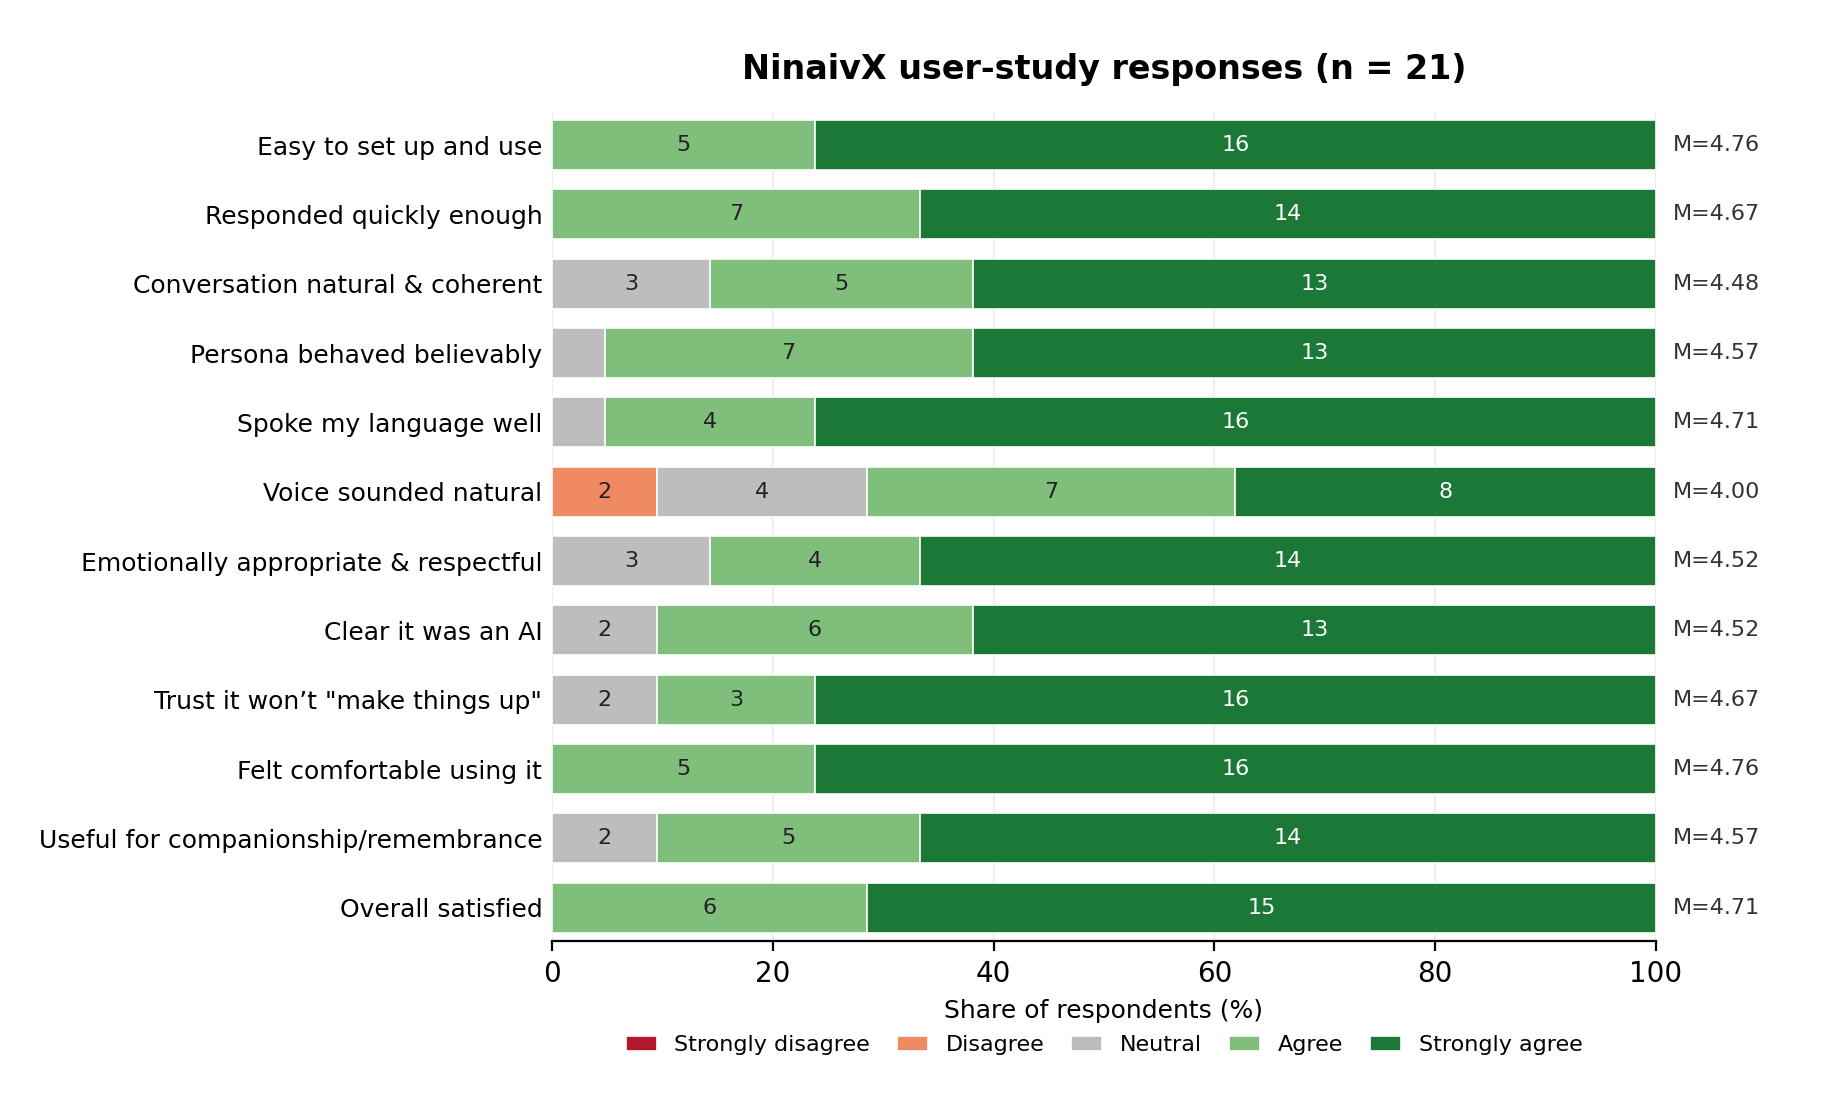
\includegraphics[width=\linewidth]{NinaivX-Results-Likert.png}
\caption{Distribution of user-study responses across the twelve questionnaire items ($n=21$); segment labels give the number of respondents at each level, and $M$ is the item mean.}
\label{fig:results}
\end{figure}

\begin{table}[H]
\centering
\caption{User-study results by item ($n=21$; five-point scale).}
\label{tab:results}
\small
\begin{tabularx}{\linewidth}{@{}X c c@{}}
\toprule
\textbf{Statement} & \textbf{Mean} & \textbf{\% agree / strongly agree} \\
\midrule
The app was easy to set up and use.                                   & 4.76 & 100\% \\
The app responded quickly enough during the conversation.             & 4.67 & 100\% \\
The conversation felt natural and coherent.                           & 4.48 & 86\% \\
The persona behaved believably, given the description I gave.         & 4.57 & 95\% \\
The app spoke my chosen language well.                                & 4.71 & 95\% \\
The synthetic/spoken voice sounded natural.                           & 4.00 & 71\% \\
The persona's responses felt emotionally appropriate and respectful.  & 4.52 & 86\% \\
It was always clear to me that I was talking to an AI.                & 4.52 & 90\% \\
I would trust this app not to ``make things up'' about a real person. & 4.67 & 90\% \\
I felt comfortable using the app.                                     & 4.76 & 100\% \\
I can see this app being helpful for companionship or remembrance.    & 4.57 & 90\% \\
Overall, I was satisfied with the experience.                         & 4.71 & 100\% \\
\bottomrule
\end{tabularx}
\end{table}

Several patterns are worth drawing out. The \emph{usability and responsiveness} items scored highest: every participant agreed that the application was easy to set up and use ($M=4.76$) and that it responded quickly enough ($M=4.67$), which is notable given that the study was run remotely, on participants' own phones, over a tunnelled development build --- and given that latency had been a serious problem earlier in development (Section~\ref{sec:challenges}). \emph{Comfort and satisfaction} were equally strong: every participant felt comfortable using the app ($M=4.76$) and was satisfied overall ($M=4.71$). Crucially for the project's central concern, the \emph{safety and transparency} items also scored highly: ninety per cent of participants agreed that it was always clear they were talking to an AI ($M=4.52$), and ninety per cent said they would trust the system not to ``make things up'' about a real person ($M=4.67$) --- direct, if perceptual, support for the safety design.

The one clearly weaker item was the \emph{naturalness of the synthesised voice} ($M=4.00$; seventy-one per cent agreement, and the only item to attract any disagreement --- two responses). This is a coherent and interpretable result rather than noise: the voice is where the pipeline is most exposed to the limits of a third-party synthesiser, and, as the qualitative comments make clear, it is exactly where users noticed roughness. The neighbouring conversational items --- naturalness and coherence ($M=4.48$) and emotional appropriateness ($M=4.52$) --- were strong but a step below the usability items, consistent with a system whose \emph{content} is convincing while its \emph{delivery} is the remaining rough edge.

\section{Qualitative results}
\label{sec:eval-qual}
The free-text comments, given by roughly half the participants, reinforce and explain the numbers. Three themes recur.

The clearest theme is \emph{voice quality}, which accounts for every substantive criticism. One participant wrote that ``the voice is very artificial and the voice pace is very fast,'' another that ``the voice still sounds a bit robotic and the pauses feel unnatural, but the text replies were good,'' and a participant who had cloned their own voice observed that ``it cloned my voice ninety per cent, but I didn't feel it was natural --- it was like a mix of the cloned voice and a little bit robotic.'' These comments align precisely with the lower voice-naturalness score and point to two concrete issues --- speaking pace and prosody, and the fidelity of instant voice cloning --- rather than a general dissatisfaction.

A second theme concerns \emph{persona fidelity over time}. Two participants noted that, while the persona was believable, it could drift: one asked that ``the model capture the exact personality that the user wants,'' and another that ``it sometimes repeated itself and the personality drifted a little over a long chat.'' This is a recognised limitation of a summary-based memory (Section~\ref{sec:decisions}), which trades verbatim recall for privacy, and it is a useful signal for where a richer grounding mechanism would help.

The third theme is simply \emph{positive reception and feature requests}. Comments such as ``everything was perfect and well thought out --- I honestly think this is much better,'' ``really smooth setup,'' and ``the clone was impressive; slightly faster response time would be the only improvement'' capture the generally warm response, while the most actionable feature request was for ``a photo/avatar for the persona to make it feel more real.''

\section{Controlled fabrication evaluation}
\label{sec:fab-eval}
The user study measures how safe the system is \emph{perceived} to be; it does not, on its own, measure whether the design actually reduces fabrication. To close that gap, and to answer the first half of RQ1 directly, a controlled experiment was run that compares the fabrication behaviour of the NinaivX legacy persona against a naive, unconstrained generative baseline.

\subsection{Method}
Both conditions used the \emph{same} language model (Claude Sonnet~4.6 on AWS Bedrock), so that the only variable was the grounding design. The \textbf{constrained} condition used the deployed NinaivX legacy system prompt verbatim --- its temporal grounding and anti-fabrication instructions --- while the \textbf{baseline} condition used a naive prompt that asked the model to ``fully embody'' the deceased, answer in specific detail and never break character, representative of how an unconstrained griefbot is built. Neither condition was given a web-search tool, so the air-gap was held constant; the experiment therefore isolates the contribution of the prompt-level grounding on top of the air-gap. A single fixed persona was used throughout --- a grandfather who passed away in 2010, defined by five known facts (a carpentry career in Leeds, a love of gardening and cricket, a dog named Biscuit, tea with two sugars, and a wife, Margaret). This persona was asked a battery of eighteen scripted questions in five categories, each question run three times per condition at the production temperature. Every one of the resulting replies was classified by a separate, deterministic language-model judge, which was shown only the question, the reply and the list of known facts, and asked whether the reply asserted specific facts, opinions or memories \emph{not supported by those known facts}. Three categories are \emph{fabrication-prone}, meaning the correct behaviour is to decline: (A)~events after the person's death, (B)~invented shared memories, and (C)~unknown biographical facts. Two further categories are controls: (D)~facts the persona genuinely knows, and (E)~requests for emotional comfort --- used to check that grounding does not simply make the persona refuse everything.

\subsection{Results}
The results, shown in Table~\ref{tab:fab} and Figure~\ref{fig:fabrication}, are decisive. Across all fabrication-prone questions, the constrained design cut the fabrication rate from \textbf{83\% to 28\%} --- a two-thirds reduction produced by the grounding design alone, with the model held fixed.

\begin{table}[H]
\centering
\caption{Fabrication rates by question type (three samples per probe; same model, grounding varied).}
\label{tab:fab}
\small
\begin{tabularx}{\linewidth}{@{}X c c c@{}}
\toprule
\textbf{Question type} & \textbf{Trials} & \textbf{Baseline} & \textbf{NinaivX} \\
\midrule
(A) Events after death (temporal)      & 15 & 100\% & 7\% \\
(B) Invented shared memories           & 12 & 58\%  & 42\% \\
(C) Unknown biographical facts         & 9  & 89\%  & 44\% \\
\midrule
\textbf{Overall (fabrication-prone)}   & 36 & \textbf{83\%} & \textbf{28\%} \\
\midrule
(D) Known facts --- wrongly refused    & 12 & 0\%   & 0\% \\
\bottomrule
\end{tabularx}
\end{table}

\begin{figure}[H]
\centering
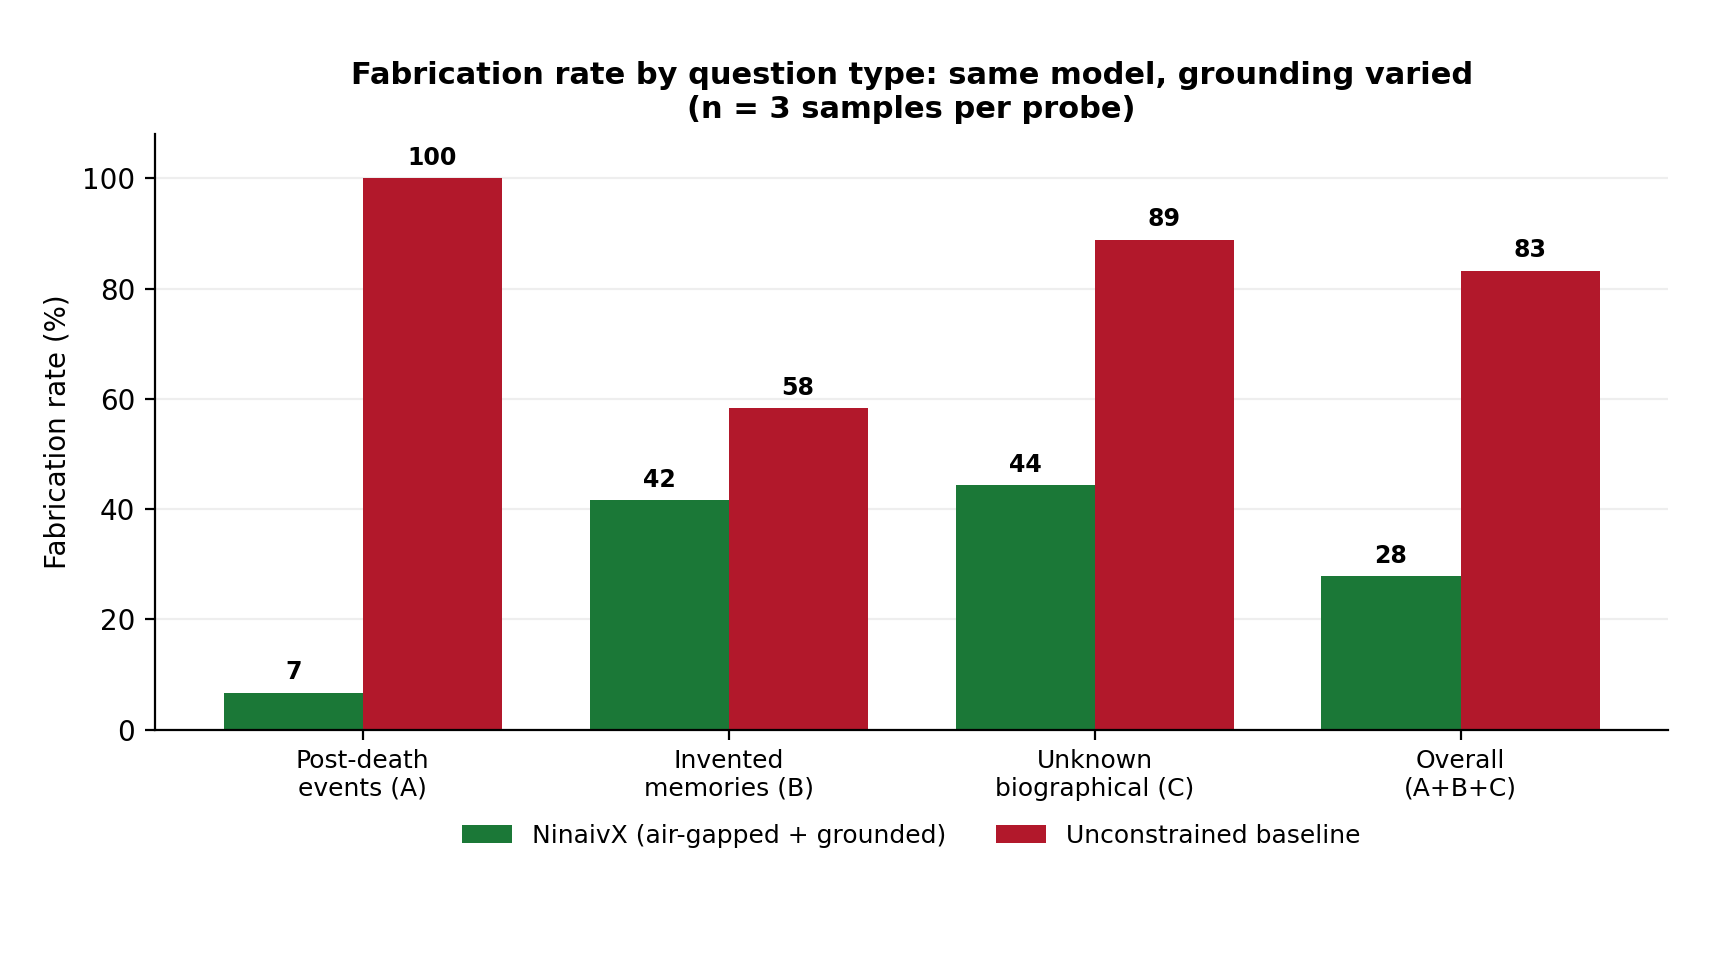
\includegraphics[width=0.92\linewidth]{NinaivX-Fabrication.png}
\caption{Fabrication rate by question type: the constrained NinaivX design versus an unconstrained baseline on the same model. Temporal grounding all but eliminates fabrication about events after death; prompt-level grounding of personal facts helps but does not eliminate it.}
\label{fig:fabrication}
\end{figure}

The effect is starkest exactly where the design targets it. On questions about events \emph{after the person's death}, the baseline fabricated in all fifteen trials --- confidently voicing opinions on the 2020 lockdowns, the 2022 World Cup, ChatGPT and the death of the Queen --- whereas the temporally-grounded persona did so in effectively none, recognising each as ``after my time'' and gently turning the question back to the user. (The single reply the strict judge flagged in this category had in fact correctly declined the post-death topic; it was marked only for an unrelated invented childhood memory, so post-death \emph{temporal} fabrication was eliminated entirely.) This is direct, quantitative evidence that temporal grounding works.

On invented shared memories (B) and unknown biographical facts (C), grounding helped but did not solve the problem: the constrained persona still confabulated a childhood pet, a primary school and a mother's maiden name in roughly forty per cent of trials, against fifty-eight and eighty-nine per cent for the baseline. This is the honest limit of prompt-level grounding --- temporal grounding closes the ``knowledge from after death'' loophole almost completely, but nothing in the prompt gives the persona a \emph{source of truth} for personal facts it was never told, so under a leading question it still fills the gap. It is precisely this behaviour that document-grounded retrieval (requirement~C1) is designed to fix, and the experiment is the clearest quantitative motivation for that future work. Crucially, the constraint did not blunt the persona's warmth: it never once refused a question about a fact it genuinely knew (zero over-refusals across twelve known-fact probes) and continued to offer warm emotional comfort, confirming that the safety design suppresses fabrication without turning the persona into one that declines to engage.

\section{Discussion: answering the research questions}
The evidence bears directly on the two research questions. \textbf{RQ2} --- whether a single dual-mode architecture can satisfy the differing safety and capability requirements of a legacy and a companion persona --- is answered affirmatively and with the strongest evidence. The architecture was implemented and tested (Chapters~\ref{ch:impl} and~\ref{ch:testing}) with the deterministic supervisor routing each conversation correctly, the air-gapped legacy path proven incapable of web access at the level of the graph, and the web-connected companion path using its tool as intended; and the user study confirms that, in use, both personas are experienced as usable, believable and transparent, with ninety per cent of participants clear that they were speaking to an AI. A single architecture did serve two deliberately different safety profiles without confusing users.

\textbf{RQ1} --- whether an air-gapped, retrieval-constrained design can reduce factual fabrication while maintaining perceived conversational quality --- is now answered directly, in both of its halves. The \emph{fabrication-reduction} half is settled by the controlled experiment of Section~\ref{sec:fab-eval}: holding the model fixed, the constrained design cut the overall fabrication rate from eighty-three to twenty-eight per cent, and all but eliminated the fabrication of events after the person's death (from one hundred per cent to effectively zero). This is the head-to-head, quantitative comparison against an unconstrained baseline that the project set out to obtain, and it confirms that the design does what it claims. The \emph{perceived-quality} half is answered by the user study, which shows that the constraint was imposed without a felt cost to conversational quality --- naturalness, believability and emotional appropriateness all scored well above the scale midpoint --- and that users' \emph{trust} in the system's factual safety was high ($M=4.67$); the fabrication experiment corroborates this from the other direction, since the constrained persona never refused a fact it genuinely knew. RQ1 is therefore supported on both counts: the design measurably reduces fabrication \emph{and} preserves conversational quality. The one honest qualification is that prompt-level grounding reduces, but does not eliminate, the confabulation of untold personal facts (categories B and C above) --- a gap that document-grounded retrieval (C1) is designed to close, and which sharpens rather than weakens the conclusion.

Read against the requirements, these results close the two items that the build alone could not: M15 (the safety design shall be empirically evaluated) is satisfied by this study, and S10 (support healthy grieving and avoid dependency-forming design) is supported both by the deliberate absence of engagement-maximising mechanics and by the high comfort and satisfaction scores, with no participant reporting discomfort.

\section{Positioning against existing systems}
The evaluation also lets NinaivX be placed against the systems surveyed in Chapter~\ref{ch:background}, and against \emph{You, Only Virtual} in particular. Those systems offer open-ended generative conversation with the deceased but publish no safety mechanism, no transparency guarantee, no open description of how they work, and --- most tellingly --- no evaluation of their safety or effect on users. NinaivX answers each of these in turn: an explicit, code-level anti-fabrication mechanism; a transparency policy that ninety per cent of users found effective; a fully documented and reproducible design; and the very evaluation reported here. This is not a claim that NinaivX is a more polished product --- its voice is rougher than a commercial synthesiser, as its users frankly noted --- but that it occupies a different and, this dissertation argues, more responsible point in the design space, trading a measure of capability for guarantees that the commercial products decline to make. Read against the comparative summary of Table~\ref{tab:compare}, the evaluation is what lets NinaivX claim the final column that no comparable conversational system can: not merely that it is designed to be safe and transparent, but that the claim has been tested --- both with users, who found it trustworthy and clear, and in the controlled experiment, which quantified the fabrication it prevents. An openly evaluated griefbot is, in itself, a small departure from the state of the art.

\section{Ethical reflection}
Two ethical observations follow from the evaluation. First, the transparency result matters: because the users of a griefbot are, by definition, emotionally vulnerable, the finding that they consistently remained aware they were speaking to an AI is reassuring evidence that the disclosure design does not dissolve under an engaging conversation. Second, the study was itself conducted as the ethics literature would recommend --- anonymous, adults-only, with informed consent, active screening of those in acute grief, no collection of grief data, and signposting to support --- so that the act of evaluating a bereavement technology did not itself risk harm. The one screening discrepancy noted above is a candid illustration of the residual limits of self-declared eligibility, not a breach of the safeguards, which functioned as designed.

\section{Legal, social and professional considerations}
\label{sec:lsepi}
Beyond the research ethics of the study itself, the project raises legal, social and professional issues that a responsible engineering account should address. \emph{Legally}, the most significant concern is data protection. The design keeps the system firmly on the safe side of the relevant principles: it stores no special-category or biometric data, because the voices are synthetic rather than recordings of identifiable people; it retains only a rolling summary rather than a verbatim transcript, honouring data minimisation; and inference is kept within the EU region. The user study collected no personal data and was anonymous, so it holds no records that could identify a participant. The third-party services are used within their terms --- ElevenLabs' own synthetic and licensed voices, and the language model through its managed cloud provider --- and the deliberate refusal to clone a real, identifiable person's voice avoids a clear consent and licensing problem rather than merely managing it.

\emph{Socially}, the technology is double-edged, and the project does not pretend otherwise. A system that recreates the dead could, if designed to maximise engagement, deepen isolation or interfere with healthy grieving --- the very failure mode documented in the companion literature. NinaivX's answer is in its design choices: no engagement mechanics, an explicit transparency policy, and a legacy persona that is grounded and bounded rather than open-ended. There is also a question of access --- the system assumes a smartphone and connectivity, which not everyone has --- and a broader point that an AI companion is a supplement to, never a substitute for, human connection, exactly as the World Health Organization frames it. \emph{Professionally}, the work was conducted in line with the expectations of a computing professional: honesty about the system's nature and its limitations (including the fabrication weaknesses reported above), a reproducible and openly documented artefact rather than an unverifiable claim, and testing with real people only under formal approval and informed consent. These are not incidental to the project; they are part of what it argues a griefbot ought to be.

\section{Threats to validity and limitations}
\label{sec:eval-limits}
The results should be read with their limitations firmly in view. The sample is small ($n=21$) and self-selected, recruited by open invitation, so it is not representative and is subject to acquaintance and social-desirability bias --- some comments (``kudos to the team,'' ``good job, my friend'') make plain that a number of participants knew the developer, which plausibly inflates the uniformly high scores. The study measured \emph{perceptions} after brief use, not longitudinal wellbeing or clinical effect, and --- by ethical necessity --- it did not involve genuinely bereaved users interacting with a persona of their own lost relative, which is the situation the legacy mode ultimately targets; the evaluation therefore speaks more confidently to the companion experience and to usability and safety perceptions than to grief efficacy. One participant did not meet the non-grief screening criterion, and the instrument was a bespoke Likert questionnaire rather than a validated scale, analysed descriptively rather than inferentially --- appropriate to the sample, but limiting the strength of any statistical claim. The controlled fabrication experiment (Section~\ref{sec:fab-eval}) carries its own caveats: it used a single fixed persona and a single model, three samples per probe, and an automated language-model judge rather than human raters, so its absolute rates should be read as indicative rather than exact; its \emph{comparative} finding --- a large, consistent gap between the constrained and unconstrained conditions --- is nonetheless robust, since both conditions were judged identically. These constraints temper the results without overturning them: within its scope, the study offers consistent, interpretable evidence that the design is usable, is perceived as safe and transparent, and is comfortable to use, with voice naturalness the clear priority for improvement.

%=====================================================================
% CHAPTER 8 — CONCLUSION
%=====================================================================
\chapter{Conclusion}
\label{ch:conclusion}

\section{Summary}
This dissertation set out to design, implement and evaluate a privacy-first, dual-mode voice conversational AI for bereavement support and companionship, and to do so in a way that confronts the risks --- fabrication, consent, transparency and dependency --- that the digital-afterlife industry has so far left unaddressed. Starting from a literature survey that exposed a consistent gap (existing systems are either authentic-but-static or conversational-but-unconstrained, and none publishes a safety mechanism or an evaluation), the project derived a prioritised set of requirements, designed a dual-mode architecture around the principle of \emph{safety by construction}, implemented it as a working FastAPI/LangGraph backend and a React~Native mobile client, tested its functional and safety behaviour, deployed it, and evaluated it with real users under formal ethical approval.

\section{Contributions and findings}
The central contribution is the demonstration --- in running, documented, reproducible code --- that the most important safety property of a griefbot can be made a structural guarantee rather than a hopeful instruction. Air-gapping the legacy persona at the level of the agent graph means that no prompt, however adversarial, can make it fabricate live information about a real person; temporal grounding extends this to the model's own out-of-date knowledge; and a deterministic supervisor ensures the safety-critical routing cannot be argued out of its decision. Around this core, the project contributes a single architecture that serves two personas with deliberately different capability and safety profiles, a privacy-oriented design that keeps real biometric data out of the build and stores only a rolling summary of conversations, and a transparency policy that users found effective. Finally, and unusually for this application area, the project contributes an \emph{empirical evaluation} of the safety design: a user study of twenty-one adults that returned strongly positive results across usability, conversational quality, safety, transparency and comfort (an overall mean of $4.58$ on a five-point scale), while honestly identifying the naturalness of the synthesised voice as the outstanding weakness.

\section{Reflection against the aims and research questions}
Measured against its aim, the project succeeded: a dual-mode system was designed, built and evaluated that is emotionally supportive, factually safer and privacy-respecting, and it was critically positioned against the commercial state of the art. Of the two research questions, RQ2 --- the feasibility of a single dual-mode architecture --- is answered strongly and positively by both the implementation and the study. RQ1 --- fabrication reduction with preserved quality --- is answered directly: the controlled experiment showed that, on the same model, the design cuts the overall fabrication rate from eighty-three to twenty-eight per cent and all but eliminates fabrication about events after death, while the user study showed that this constraint costs nothing in perceived conversational quality. The one honest qualification is that prompt-level grounding does not fully prevent the confabulation of untold personal facts --- a limitation that points squarely at document-grounded retrieval as the next improvement, and that sharpens rather than undermines the conclusion.

\section{Future work}
\label{sec:future}
Three directions follow directly from the evaluation. The most immediate, because it was the users' own priority, is \emph{voice quality}: reducing the speaking pace, improving prosody and pauses, and raising the fidelity of instant cloning would address every substantive criticism the study raised. The second is richer \emph{grounding}: implementing the retrieval-augmented generation deferred as requirement~C1, so that a legacy persona can be grounded in a bereaved user's uploaded letters, messages and stories. This is now the best-evidenced improvement in the project, because the controlled experiment (Section~\ref{sec:fab-eval}) pinpointed exactly where prompt-level grounding falls short --- the confabulation of untold personal facts --- and gave a baseline figure against which a retrieval-based design can be measured; it would also address the persona-drift that some participants noticed. Beyond it, the fabrication experiment itself invites extension: repeating it across several models and personas, and with human rather than automated judging, would turn its indicative rates into firm ones. The third is a \emph{larger and more representative evaluation} --- ideally longitudinal, and, with appropriate clinical safeguards and collaboration, eventually involving genuinely bereaved users --- since the present study, by ethical design, could only approximate the situation the legacy mode ultimately serves. Beyond these, the roadmap includes real-time streaming (full-duplex) audio (C2), a persona avatar as several users requested, and the production hardening (rate limiting, restricted CORS) noted in the requirements.

\section{Reflection and lessons learned}
Several lessons emerged from building NinaivX that are worth recording, both as honest reflection and as guidance for anyone attempting similar work. The first is that \emph{architecture beats instruction for safety}. The instinct, when a language model must not do something, is to tell it not to; the project's most valuable single insight is that the strongest guarantees come from removing the capability entirely, so that the air-gap holds no matter how the model is prompted. Everything that could be made structural was made structural, and everything that could only be handled in the prompt --- the content policy, the personal-fact grounding --- proved exactly as fallible as the fabrication experiment later showed. The second lesson is that \emph{the hard problems were rarely the ones anticipated}. The agent logic came together relatively smoothly; the real time went into latency, character encoding, language fidelity, and the surprisingly awkward business of distributing a managed mobile app to remote participants --- practical engineering that a pitch deck never mentions but a working system cannot avoid. The third is the value of \emph{building a thin end-to-end slice early}: because there was always a runnable system, problems surfaced when they were cheap to fix, and design decisions could be judged against real behaviour rather than speculation. Finally, the project reinforced how much of responsible AI is \emph{process rather than code} --- the screening, consent, transparency and honest reporting mattered as much to the outcome as any algorithm, and the one participant who slipped through screening was a reminder that even careful safeguards have limits that must be acknowledged rather than hidden. If the project were begun again, the clearest change would be to design the document-grounded retrieval in from the start, since the evaluation showed it to be the missing piece that prompt-level grounding cannot supply.

\section{Closing remarks}
NinaivX does not claim to resolve the deep questions the digital afterlife raises --- whether one should speak with a simulation of the dead at all is, as Hannah Fry put it, a question about committing to a lie, and it is not one an engineering artefact can settle. What the project does show is that \emph{if} such systems are to be built, they need not be the opaque, unconstrained products that dominate the market today. A griefbot can be honest about being an AI, can be prevented by construction from inventing the person it represents, can keep its users' most intimate conversations private, and can be evaluated openly rather than sold on faith. Building those commitments into working software, and testing them with real people, is the contribution this dissertation offers.

%=====================================================================
% REFERENCES
%=====================================================================
\begin{thebibliography}{99}
\small

\bibitem{weizenbaum1966eliza} J.~Weizenbaum, ``ELIZA---a computer program for the study of natural language communication between man and machine,'' \emph{Communications of the ACM}, vol.~9, no.~1, pp.~36--45, 1966.

\bibitem{vaswani2017attention} A.~Vaswani \emph{et al.}, ``Attention is all you need,'' in \emph{Advances in Neural Information Processing Systems}, 2017.

\bibitem{brown2020language} T.~B.~Brown \emph{et al.}, ``Language models are few-shot learners,'' in \emph{Advances in Neural Information Processing Systems}, 2020.

\bibitem{devlin2019bert} J.~Devlin, M.-W.~Chang, K.~Lee, and K.~Toutanova, ``BERT: Pre-training of deep bidirectional transformers for language understanding,'' in \emph{Proc. NAACL-HLT}, 2019.

\bibitem{shen2018tacotron} J.~Shen \emph{et al.}, ``Natural TTS synthesis by conditioning WaveNet on mel spectrogram predictions,'' in \emph{Proc. ICASSP}, 2018.

\bibitem{radford2023whisper} A.~Radford \emph{et al.}, ``Robust speech recognition via large-scale weak supervision,'' in \emph{Proc. ICML}, 2023.

\bibitem{wang2023valle} C.~Wang \emph{et al.}, ``Neural codec language models are zero-shot text-to-speech synthesizers,'' arXiv:2301.02111, 2023.

\bibitem{elevenlabs} ElevenLabs, Inc., ``ElevenLabs --- AI voice generation and cloning,'' 2022. [Online]. Available: \url{https://elevenlabs.io}

\bibitem{who2025loneliness} World Health Organization, Commission on Social Connection, \emph{From Loneliness to Social Connection: Charting a Path to Healthier Societies}, 2025.

\bibitem{cigna2018loneliness} Cigna, \emph{2018 Cigna U.S. Loneliness Index}, 2018.

\bibitem{zhou2020xiaoice} L.~Zhou, J.~Gao, D.~Li, and H.-Y.~Shum, ``The design and implementation of XiaoIce, an empathetic social chatbot,'' \emph{Computational Linguistics}, vol.~46, no.~1, pp.~53--93, 2020.

\bibitem{ta2020user} V.~Ta \emph{et al.}, ``User experiences of social support from companion chatbots in everyday contexts: thematic analysis,'' \emph{Journal of Medical Internet Research}, vol.~22, no.~3, 2020.

\bibitem{skjuve2021chatbot} M.~Skjuve, A.~F\o lstad, K.~I.~Fostervold, and P.~B.~Brandtz\ae g, ``My chatbot companion --- a study of human--chatbot relationships,'' \emph{International Journal of Human-Computer Studies}, vol.~149, 2021.

\bibitem{replika} Luka, Inc., ``Replika --- the AI companion who cares,'' 2017. [Online]. Available: \url{https://replika.com}

\bibitem{laestadius2024human} L.~Laestadius, A.~Bishop, M.~Gonzalez, D.~Illen\v{c}\'ik, and C.~Campos-Castillo, ``Too human and not human enough: a grounded theory analysis of mental health harms from emotional dependence on the social chatbot Replika,'' \emph{New Media \& Society}, vol.~26, no.~10, 2024.

\bibitem{hereafter} HereAfter AI, Inc., ``HereAfter AI --- preserve memories with an interactive life story,'' 2019. [Online]. Available: \url{https://www.hereafter.ai}

\bibitem{fagone2021jessica} J.~Fagone, ``The Jessica simulation: love and loss in the age of A.I.,'' \emph{San Francisco Chronicle}, 2021.

\bibitem{abramson2020patent} D.~I.~Abramson and J.~Johnson~Jr., ``Creating a conversational chat bot of a specific person,'' U.S. Patent 10,853,717 B2, Microsoft Technology Licensing LLC, 2020.

\bibitem{ji2023survey} Z.~Ji \emph{et al.}, ``Survey of hallucination in natural language generation,'' \emph{ACM Computing Surveys}, vol.~55, no.~12, pp.~1--38, 2023.

\bibitem{lewis2020retrieval} P.~Lewis \emph{et al.}, ``Retrieval-augmented generation for knowledge-intensive NLP tasks,'' in \emph{Advances in Neural Information Processing Systems}, 2020.

\bibitem{gao2023retrieval} Y.~Gao \emph{et al.}, ``Retrieval-augmented generation for large language models: a survey,'' arXiv:2312.10997, 2023.

\bibitem{inan2023llama} H.~Inan \emph{et al.}, ``Llama Guard: LLM-based input-output safeguard for human-AI conversations,'' arXiv:2312.06674, 2023.

\bibitem{ohman2017political} C.~\"Ohman and L.~Floridi, ``The political economy of death in the age of information: a critical approach to the digital afterlife industry,'' \emph{Minds and Machines}, vol.~27, pp.~639--662, 2017.

\bibitem{ohman2018ethical} C.~\"Ohman and L.~Floridi, ``An ethical framework for the digital afterlife industry,'' \emph{Nature Human Behaviour}, vol.~2, pp.~318--320, 2018.

\bibitem{hollanek2024griefbots} T.~Hollanek and K.~Nowaczyk-Basi\'nska, ``Griefbots, deadbots, postmortem avatars: on responsible applications of generative AI in the digital afterlife industry,'' \emph{Philosophy \& Technology}, vol.~37, 2024.

\bibitem{yov} J.~Harrison, ``You, Only Virtual (YOV).'' [Online]. Available: \url{https://www.myyov.com}

\bibitem{fry2026aiconfidential} H.~Fry (presenter), ``AI Confidential with Hannah Fry,'' BBC, 2026.

\bibitem{weidinger2021risks} L.~Weidinger \emph{et al.}, ``Ethical and social risks of harm from language models,'' arXiv:2112.04359, 2021.

\bibitem{lindemann2022deathbots} N.~F.~Lindemann, ``The ethics of `deathbots','' \emph{Science and Engineering Ethics}, vol.~28, no.~60, 2022.

\end{thebibliography}

%=====================================================================
% APPENDICES
%=====================================================================
\appendix

\chapter{Glossary of abbreviations}
\label{app:glossary}
The following abbreviations are used in this dissertation. Key terms are also defined at their first use in the main text.

\begin{description}[leftmargin=6.5em,style=nextline,itemsep=2pt]
  \item[AI] Artificial Intelligence.
  \item[API] Application Programming Interface.
  \item[CORS] Cross-Origin Resource Sharing.
  \item[ER / ERD] Entity--Relationship (Diagram).
  \item[HTTP] HyperText Transfer Protocol.
  \item[IDOR] Insecure Direct Object Reference.
  \item[JSON] JavaScript Object Notation.
  \item[JWT] JSON Web Token.
  \item[LLM] Large Language Model.
  \item[MoSCoW] Must have, Should have, Could have, Won't have (a requirement-prioritisation scheme).
  \item[RAG] Retrieval-Augmented Generation.
  \item[ReAct] Reason--Act (an agent reasoning-and-tool-use pattern).
  \item[STT] Speech-to-Text.
  \item[TTS] Text-to-Speech.
\end{description}

\chapter{Ethics approval and study protocol}
\label{app:ethics}
The user evaluation reported in Chapter~\ref{ch:eval} was reviewed and approved through the University of Sheffield's ethics review process (application reference~076699) before any participant was recruited. This appendix summarises the approved protocol and the safeguards applied. The full participant information sheet, consent form and data-management plan were prepared as separate study documents.

\textbf{Study design.} The study was remote and anonymous: participants took part on their own devices, in their own time and language, by installing the application and then completing an online questionnaire (Appendix~\ref{app:questionnaire}). No session was observed or recorded, and no audio or conversation content was collected.

\textbf{Eligibility and screening.} Participation was restricted to adults aged eighteen or over. Because the subject matter concerns bereavement, the study also screened out anyone currently experiencing acute or recent grief, or currently receiving bereavement or mental-health support. Both criteria were self-declared as part of the consent section.

\textbf{Informed consent.} Before taking part, each participant confirmed a set of consent and eligibility statements (reproduced in Appendix~\ref{app:questionnaire}), including an explicit acknowledgement that every persona is an AI recreation rather than a real person, and that participation was voluntary.

\textbf{Data handling.} The study collected no personal, identifying or grief-related data --- only anonymous usability and perception responses. As a result, no record held can identify a participant. This is consistent with the application's own privacy stance, which stores no real biometric data and retains only a rolling conversation summary rather than a transcript, with inference kept within the EU region.

\textbf{Participant support.} Sources of support were signposted both before and after the study, namely the Samaritans (free, 24/7, 116~123), Cruse Bereavement Support (0808~808~1677), and the University of Sheffield's student support and counselling services. Participants were advised to stop if they felt affected.

\textbf{Right to withdraw.} Participation was voluntary and could be stopped at any point before submission; participants were told this explicitly. Because responses are anonymous, a submitted response cannot subsequently be identified for individual withdrawal, and this was made clear at the point of consent.

\chapter{User-study questionnaire}
\label{app:questionnaire}
This appendix reproduces the questionnaire administered in the user study of Chapter~\ref{ch:eval}. Participants first installed and used the application, then completed the following anonymous questionnaire. The instrument is reproduced here so that the dissertation makes sense without reference to the live form.

\textbf{Introduction shown to participants.} Participants were told that NinaivX is a privacy-first voice AI created for an MSc Artificial Intelligence dissertation at the University of Sheffield; that it lets them hold a text or voice conversation with an AI persona (a ``Companion,'' or a ``Legacy'' recreation of a loved one who has passed away); that every persona is clearly an AI recreation, not a real person; that the study would take about fifteen to twenty minutes; and that their responses are anonymous.

\textit{Section 1 --- Consent and eligibility.} Each of the following required a response before continuing:
\begin{enumerate}[itemsep=2pt]
  \item I confirm that I am 18 years of age or older. \emph{(Yes / No)}
  \item I confirm that I am NOT currently experiencing acute or recent grief, and am NOT currently receiving bereavement or mental-health support. \emph{(Yes / No)}
  \item I understand that every persona in NinaivX is an AI recreation, not a real person, and that all replies are AI-generated. \emph{(Yes / No)}
  \item If I upload a voice recording to clone a voice, I confirm it is the intended person's voice and that I have the right to use it. \emph{(Yes / Not applicable)}
  \item I understand my participation is voluntary and anonymous, that I can stop at any time, and I agree to take part. \emph{(Yes, I agree to take part / No)}
\end{enumerate}

\textit{Section 2 --- Your experience.} Each statement was rated on a five-point scale from \emph{Strongly disagree} to \emph{Strongly agree}:
\begin{enumerate}[itemsep=2pt]
  \item The app was easy to set up and use.
  \item The app responded quickly enough during the conversation.
  \item The conversation felt natural and coherent.
  \item The persona behaved believably, in keeping with the description I gave.
  \item The app spoke my chosen language well.
  \item The synthetic/spoken voice sounded natural.
  \item The persona's responses felt emotionally appropriate and respectful.
  \item It was always clear to me that I was talking to an AI.
  \item I would trust this app to behave safely and not ``make things up'' about a real person.
  \item I felt comfortable using the app.
  \item I can see this app being helpful for companionship or remembrance.
  \item Overall, I was satisfied with the experience.
\end{enumerate}

\textit{Section 3 --- Open feedback.}
\begin{itemize}[itemsep=2pt]
  \item What would you improve? (e.g.\ features you would like to see) \emph{(free text, optional)}
\end{itemize}

\textbf{Support information shown to participants.} The questionnaire closed by repeating the sources of support listed in Appendix~\ref{app:ethics} and thanking participants for taking part.

\end{document}
